%%%%%%%%%%%%%%%%%%%%%%%%%%%%%%%%%%%%%%%%%%%%%%%%%%%%%%%%%%%%%%%%%%%%%%%%%%%%%%%%%%%%%%%%%%%%%%
%
%                                                       Example IS Template
%
% \documentclass{woosterthesis} must be at the beginning of every IS. Options are the same as
% for the report class with some additional options, abstractonly, blacklinks, code, kaukecopyright, palatino, picins,
% maple, index, verbatim, dropcaps, euler, gauss, alltt,  woolshort, colophon, woosterchicago, and
% achemso. The kaukecopyright option will put the arch symbol with the word mark on the
% copyright page. The woosterthesis class is based on the report class. One thing to note is that
% the ``%'' symbol comments out all characters that follow it on the line.
%%%%%%%%%%%%%%%%%%%%%%%%%%%%%%%%%%%%%%%%%%%%%%%%%%%%%%%%%%%%%%%%%%%%%%%%%%%%%%%%%%%%%%%%%%%%%%

%%%%%%%%%%%%%%%%%%%%%%%%%%%%%%%%%%%%%%%%%%%%%%%%%%%%%%%%%%%%%%%%%%%%%%%%%%%%%%%%%%%%%%%%%%%%%%
% use this declaration for a draft  version of your IS
\documentclass[10pt,palatino,code,picins,kaukecopyright,openright,woolshort,dropcaps,verbatim,index,euler]{woosterthesis}
%\documentclass[10pt,code,picins,kaukecopyright,openright,woolshort,dropcaps,verbatim,euler,index,colophon,blacklinks,twoside]{woosterthesis}
% note that you can specify the woosterchicago option to use Chicago citation style and achemso to use the American Chemical Society citation format
%
%%%%%%%%%%%%%%%%%%%%%%%%%%%%%%%%%%%%%%%%%%%%%%%%%%%%%%%%%%%%%%%%%%%%%%%%%%%%%%%%%%%%%%%%%%%%%%
% use this declaration for the print version of your IS
%\documentclass[12pt,code,palatino,picins,blacklinks,kaukecopyright,openright,twoside]{woosterthesis} % probably what most students would use
%
%%%%%%%%%%%%%%%%%%%%%%%%%%%%%%%%%%%%%%%%%%%%%%%%%%%%%%%%%%%%%%%%%%%%%%%%%%%%%%%%%%%%%%%%%%%%%%
% use this declaration for the CD version of your IS
%\documentclass[12pt,code,palatino,picins,kaukecopyright,openright,twoside]{woosterthesis}
%%%%%%%%%%%%%%%%%%%%%%%%%%%%%%%%%%%%%%%%%%%%%%%%%%%%%%%%%%%%%%%%%%%%%%%%%%%%%%%%%%%%%%%%%%%%%%

%%%%%%%%%%%%%%%%%%%%%%%%%%%%%%%%%%%%%%%%%%%%%%%%%%%%%%%%%%%%%%%%%%%%%%%%%%%%%%%%%%%%%%%%%%%%%%
%
%                                                       Load Packages
%
%   To load packages in addition to the ones that are loaded by default, please place your
%   usepackage commands in the packages.tex file in the styles folder.
%
%
%%%%%%%%%%%%%%%%%%%%%%%%%%%%%%%%%%%%%%%%%%%%%%%%%%%%%%%%%%%%%%%%%%%%%%%%%%%%%%%%%%%%%%%%%%%%%%

%%%%%%%%%%%%%%%%%%%%%%%%%%%%%%%%%%%%%%%%%%%%%%%%%%%%%%%%%%%%%%%%%%%%%%%%%%%%%%%%%%%%%%%%%%%%%%
%
%                                                       Packages
%
% Do not add any other packages without consulting with Dr. Breitenbucher as they may break the functionality of the class.
%
%%%%%%%%%%%%%%%%%%%%%%%%%%%%%%%%%%%%%%%%%%%%%%%%%%%%%%%%%%%%%%%%%%%%%%%%%%%%%%%%%%%%%%%%%%%%%%

\ifxetex%
	\defaultfontfeatures{Mapping=tex-text}%
		\setmainfont[Numbers=OldStyle,BoldFont={* Semibold}]{Adobe Garamond Pro}% select the body font other choices would be Baskerville, Optima Regular, Didot, Georgia, Cochin
                      \setmathrm{Adobe Garamond Pro}
                      \setmathfont[Digits,Latin]{Adobe Garamond Pro}
		\setsansfont[Scale=.87,Fractions=On,Numbers=Lining]{Myriad Pro}% select the sans serif font other choices would be Skia, Arial, Helvetica, Helvetica Neue
%		\setmonofont[Scale=.88,Fractions=On]{Prestige Elite Std Bold}% set the mono font other choices would be Courier, Monaco, American Typewriter
	           \setmonofont[Scale=.9]{Courier Std}%
%	    \setromanfont[Fractions=On,Numbers=OldStyle, BoldFont={Warnock Pro Semibold}]{Warnock Pro}%
%	    \setsansfont[Scale=.95,Fractions=On,Numbers=Lining]{Myriad Pro}%
%	    \setmonofont[Scale=.91,Fractions=On]{Courier Std Medium}%
%	    \setmonofont[Scale=.88,Fractions=On]{American Typewriter}%
%		\setmonofont[Scale=.94,Fractions=On]{Prestige Elite Std Bold}
%    		\setromanfont[Fractions=On,Numbers=OldStyle]{Minion Pro}
 %    	\setsansfont[Scale=.9,Fractions=On,Numbers=Lining]{Myriad Pro}
%     	\setmonofont[Scale=.93,Fractions=On]{Courier Std Medium}
%     	\setromanfont[Fractions=On,Numbers=OldStyle]{Minion Pro}
%     	\setsansfont[Scale=.85,Fractions=On,Numbers=Lining]{News Gothic Std}
%    		\setmonofont[Scale=.93,Fractions=On]{Prestige Elite Std}
%		\setromanfont[Fractions=On,Numbers=OldStyle]{Minion Pro}
%		\setsansfont[Scale=.9,Fractions=On,Numbers=Lining]{Bell Gothic Std Bold}
%		\setmonofont[Scale=.95,Fractions=On]{Prestige Elite Std Bold}
\fi

%%%%%%%%%%%%%%%%%%%%%%%%%%%%%%%%%%%%%%%%%%%%%%%%%%%%%%%%%%%%%%%%%%%%%%%%%%%%%%%%%%%%%%%%%%%%%%
%
%                                                       Load Personal commands
%                                                                    
% There will be certain commands that you use frequently in the thesis. You can give these
% commands new names which are easier for you to remember. You can also combine several
% commands into a new command of your own. See The LaTeX Companion or Guide to LaTeX
% for examples on defining your own commands. These are commands that I defined to cut
% down on typing. You can enter your commands in the personal.tex file in the styles folder.
%
%%%%%%%%%%%%%%%%%%%%%%%%%%%%%%%%%%%%%%%%%%%%%%%%%%%%%%%%%%%%%%%%%%%%%%%%%%%%%%%%%%%%%%%%%%%%%%

%%%%%%%%%%%%%%%%%%%%%%%%%%%%%%%%%%%%%%%%%%%%%%%%%%%%%%%%%%%%%%%%%%%%%%%%%%%%%%%%%%%%%%%%%%%%%%
%
%                                                       Personal Commands
%                                                                    
% There will be certain commands that you use frequently in the thesis. You can give these
% commands new names which are easier for you to remember. You can also combine several
% commands into a new command of your own. See The LaTeX Companion or Guide to LaTeX for
% examples on defining your own commands. These are commands that I defined to cut down on typing.
%
%%%%%%%%%%%%%%%%%%%%%%%%%%%%%%%%%%%%%%%%%%%%%%%%%%%%%%%%%%%%%%%%%%%%%%%%%%%%%%%%%%%%%%%%%%%%%%

\newcommand{\fl}{\ell}
\newcommand{\lt}{\LaTeX\ }
\newcommand{\msw}{Word\texttrademark\ }
\newcommand{\xt}{\ifthenelse{\boolean{xetex}}{\XeTeX\ }{XeTeX} }
%\newcommand{\Cl}{\ensuremath{\textup{C}_\fl}}
%\newcommand{\bCl}{C$_{\ell}$}
%\newcommand{\Al}{\ensuremath{\textup{A}_\fl}}
%\newcommand{\msum}{{(m_1+\cdots+m_\ell)}}
%\newcommand{\Nsum}{{(N_1+\cdots+N_\ell)}}
%\newcommand{\ysum}{{(y_1+\cdots+y_\ell)}}
%\newcommand{\Nsub}{{N_1+\cdots+N_\ell}}
%\newcommand{\ysub}{{y_1+\cdots+y_\ell}}
%\newcommand{\xsub}{{x_1+\cdots+x_\ell}}
%\newcommand{\ysqsum}{{y_1^2+\cdots +y_{\fl}^2}}
%\newcommand{\msqsum}{{m_1^2+\cdots +m_{\fl}^2}}
%\newcommand{\ratio}{\left(\frac{\beta}{\alpha}\right)}
%\newcommand{\LT}{\ensuremath{\LaTeX{}}}

%%%%%%%%%%%%%%%%%%%%%%%%%%%%%%%%%%%%%%%%%%%%%%%%%%%%%%%%%%%%%%%%%%%%%%%%%%%%%%%%%%%%%%%%%%%%%%
% These commands have one argument and are entered as \commandname{argument}.
%%%%%%%%%%%%%%%%%%%%%%%%%%%%%%%%%%%%%%%%%%%%%%%%%%%%%%%%%%%%%%%%%%%%%%%%%%%%%%%%%%%%%%%%%%%%%%

%\newcommand{\bd}[1]{\textbf{#1}}
\newcommand{\mbd}[1]{{\mathbf{#1}}}
%\newcommand{\abs}[1]{\vert{#1}\vert}
\newcommand{\bvec}[1]{{\mbd{#1}}}
%\newcommand{\lvec}[1]{\abs{\bvec{#1}}}
%\newcommand{\nesmallprod}[1]{\prod_{\substack{#1=1\\
%#1\neq p}}^{\fl}}
%\newcommand{\esec}[1]{e_{2}({#1}_1,\ldots ,{#1}_\fl)}
%\newcommand{\smallprod}[1]{\prod_{#1=1}^{\fl}}
%\newcommand{\incsum}[1]{{#1}_2+2{#1}_3+\cdots +(\fl -1){#1}_\fl}
%\newcommand{\binomsum}[1]{\binom{{#1}_1}{2}+\cdots +\binom{{#1}_\fl}{2}}
%\newcommand{\imultsum}[1]{\multsum{{#1}_k\ge 0}{k=1,\ldots ,\fl}}
%\newcommand{\diagsum}[1]{\sum _{\substack{{#1}_k\ge 0\\
%k=1, \ldots ,\fl\\
%\lvec{#1}=m}}}
%\newcommand{\Mb}[1][\fl]{\ensuremath{\textup{\bd{M}}_b^{(#1)}}}
%\newcommand{\HLV}[1]{\ensuremath{\textup{\bd{H}}_{#1}}}
%\newcommand{\Rq}[1][p]{\ensuremath{\textup{R}_q^{(#1)}}}
\newcommand{\degree}[1]{\ensuremath{#1^{\circ}}}
\newcommand{\ip}[1]{\texttt{#1}\index{packages!#1}}
\newcommand{\ic}[1]{\texttt{$\backslash$#1}\index{commands!#1}}
\newcommand{\ie}[1]{#1\index{#1}}

%%%%%%%%%%%%%%%%%%%%%%%%%%%%%%%%%%%%%%%%%%%%%%%%%%%%%%%%%%%%%%%%%%%%%%%%%%%%%%%%%%%%%%%%%%%%%%
% These commands have 2 or more arguments some with default values for the first argument. You
% can learn a lot about constructing complicated equations by studying the commands in this %section.
%%%%%%%%%%%%%%%%%%%%%%%%%%%%%%%%%%%%%%%%%%%%%%%%%%%%%%%%%%%%%%%%%%%%%%%%%%%%%%%%%%%%%%%%%%%%%%

%\newcommand{\qbinom}[2]{\ensuremath{\left[{#1}\atop{#2}\right]_q}}
%\newcommand{\sqprod}[2]{\prod_{#1,#2=1}^{\fl}}
%\newcommand{\triprod}[2]{\prod_{1\le #1<#2\le \fl}}
%\newcommand{\nesqprod}[2]{\prod_{\substack{#1,#2=1\\
%#1,#2\neq p}}^{\fl}}
%\newcommand{\netriprod}[2]{\prod_{\substack{1\le #1<#2\le \fl\\
%#1,#2\neq p}}}
\newcommand{\qrfac}[3][\ ]{\left({#2}\right)_{#3}^{#1}}
%\newcommand{\multsum}[2]{\sum_{\substack{{#1}\\
%\\
%{#2}}}}
%\newcommand{\fmultsum}[2][N]{\multsum{0\le {{#2}_k}\le {{#1}_k}}{k=1,\ldots ,\fl}}
%\newcommand{\pq}[2]{\ _{#1}\varphi_{#2}}
%\newcommand{\mess}[2][y_k]{\frac{\qrfac{\alpha x_k}{#2}\qrfac{qx_k\beta^{-1}}{#2}}{\qrfac{\beta x_k}{#1}
%\qrfac{qx_k\alpha^{-1}}{#1}}}
%\newcommand{\MG}[7][\fl]{\ensuremath{\left[\textup{MG}\right]_{#2}^{(#1)}{#3}q;{#4};{#5}^{#6}{#7}}}

%%%%%%%%%%%%%%%%%%%%%%%%%%%%%%%%%%%%%%%%%%%%%%%%%%%%%%%%%%%%%%%%%%%%%%%%%%%%%%%%%%%%%%%%%%%%%%
% These commands define new environments
%%%%%%%%%%%%%%%%%%%%%%%%%%%%%%%%%%%%%%%%%%%%%%%%%%%%%%%%%%%%%%%%%%%%%%%%%%%%%%%%%%%%%%%%%%%%%%

\newcounter{unnumft}
\setcounter{unnumft}{0}
\newenvironment{unnumft}[2]{\renewcommand{\thefootnote}{}\footnote{#1}\footnote{#2}} {\addtocounter{footnote}{-2}}
\newenvironment{wooexample}{\small
\begin{singlespace}
\begin{example}}{\end{example}
\end{singlespace}}

\graphicspath{{./figures/}}% for setting where to look for figures
\citestyle{wooster}% change the style of citations. Math and CS people should leave this alone.






%%%%%%%%%%%%%%%%%%%%%%%%%%%%%%%%%%%%%%%%%%%%%%%%%%%%%%%%%%%%%%%%%%%%%%%%%%%%%%%%%%%%%%%%%%%%%%
%
%                                                       Load Theorem formatting information
%
%  If you need to define an new theorem style or want to see what theorem like environments 
%  are available please look at the theorems.tex file in the styles folder.
%
%%%%%%%%%%%%%%%%%%%%%%%%%%%%%%%%%%%%%%%%%%%%%%%%%%%%%%%%%%%%%%%%%%%%%%%%%%%%%%%%%%%%%%%%%%%%%%

%%%%%%%%%%%%%%%%%%%%%%%%%%%%%%%%%%%%%%%%%%%%%%%%%%%%%%%%%%%%%%%%%%%%%%%%%%%%%%%%%%%%%%%%%%%%%%
%
% This is where one would tell \LaTeX{} how to format Theorems, Definitions, etc. and also
% indicate the environment names. You need the amsthm package (loaded in the woosterthesis %class) in order for these commands to work.
%
%%%%%%%%%%%%%%%%%%%%%%%%%%%%%%%%%%%%%%%%%%%%%%%%%%%%%%%%%%%%%%%%%%%%%%%%%%%%%%%%%%%%%%%%%%%%%%

% an example of defining your own theoremstyle
%\newtheoremstyle{break}% name
%  {\topsep}%      Space above
%  {\topsep}%      Space below
%  {\itshape}%         Body font
%  {}%         Indent amount (empty = no indent, \parindent = para indent)
%  {\bfseries}% Thm head font
%  {.}%        Punctuation after thm head
%  {\newline}%     Space after thm head: " " = normal interword space;
%        %       \newline = linebreak
%  {}%         Thm head spec (can be left empty, meaning `normal')
\newtheoremstyle{scthm}{\topsep}{\topsep}{\itshape}{}{\bfseries\scshape}{}{ }{}% small cap font for the heading
\newtheoremstyle{itdefn}{\topsep}{\topsep}{\itshape}{}{\bfseries}{.}{ }{}% italic definitions
\newtheoremstyle{scdefn}{\topsep}{\topsep}{\itshape}{}{}{}{ }{\thmname{\textbf{#1}}\thmnumber{ \textbf{#2}}\thmnote{ \scshape #3:}}% small cap headings and italic text.

\theoremstyle{break}% this theoremstyle will put the text of the theorem on a new line.
\newtheorem{thm}{Theorem}[chapter]%number theorems within chapters 
%\newtheorem{cor}[thm]{Corollary}%by using [thm] we are numbering these environments with the theorems.
\newtheorem{cor}{Corollary}[chapter]%number corollaries within chapters .
%\newtheorem{lem}[thm]{Lemma}
\newtheorem{lem}{Lemma}[chapter]
%\newtheorem{prop}[thm]{Proposition}
\newtheorem{prop}{Proposition}[chapter]

\theoremstyle{scdefn}
%\newtheorem{defn}[thm]{Definition}
\newtheorem{defn}{Definition}[chapter]
\theoremstyle{remark}
%\newtheorem{rem}[thm]{Remark}
\newtheorem{rem}{Remark}[chapter]
\renewcommand{\therem}{}
%\newtheorem{ex}[thm]{Example}
\newtheorem{ex}{Example}[chapter]

\theoremstyle{plain}
%\newtheorem{note}[thm]{Notation}
\newtheorem{note}{Notation}[chapter]
\renewcommand{\thenote}{}
%\newtheorem{nts}[thm]{Note to self}%use to remind yourself of things yet to do
\newtheorem{nts}{Note to self}[chapter]
\renewcommand{\thents}{}
%\newtheorem{terminology}[thm]{Terminology}
\newtheorem{terminology}{Terminology}[chapter]
\renewcommand{\theterminology}{}

\theoremstyle{itdefn}
\newtheorem{bdefn}{Definition}[chapter]
\newsavebox{\fmbox} 
\newenvironment{boxeddefn}[2] 
{\begin{lrbox}{\fmbox}\begin{minipage}{0.9 \linewidth }\begin{singlespace}\begin{bdefn}[{#1}]\label{#2}\vspace{0.2cm}} 
{\end{bdefn}\end{singlespace}\end{minipage}\end{lrbox}\fbox{\usebox{\fmbox}}}

\setcounter{secnumdepth}{5}% controls the numbering of sections
\setcounter{tocdepth}{6}% controls the number of levels in the Contents

%%%%%%%%%%%%%%%%%%%%%%%%%%%%%%%%%%%%%%%%%%%%%%%%%%%%%%%%%%%%%%%%%%%%%%%%%%%%%%%%%%%%%%%%%%%%%%
% This is where one enters the information about the thesis.
%%%%%%%%%%%%%%%%%%%%%%%%%%%%%%%%%%%%%%%%%%%%%%%%%%%%%%%%%%%%%%%%%%%%%%%%%%%%%%%%%%%%%%%%%%%%%%


\title{Grasping the Void: Immersion tactics using gesture controlled interaction systems in virtual reality.}
\thesistype{Independent Study Thesis} 
\author{Avery Rapson}
%\presentdegrees{Ph.D.} % you should comment this line
\degreetoobtain{Bachelor of Arts In Computer Science}
\presentschool{The College of Wooster}
\academicprogram{Department of Mathematics and Computer Science}
\gradyear{2017}
\advisor{Denise Byrnes, Ph.D}
%\reader{Reader}
\copyrighted   
%\copyrightdate{}                  
\makeindex % comment this line if you do not have an index

%%%%%%%%%%%%%%%%%%%%%%%%%%%%%%%%%%%%%%%%%%%%%%%%%%%%%%%%%%%%%%%%%%%%%%%%%%%%%%%%%%%%%%%%%%%%%%
% This is where the commands for the document begin. All \LaTeX{} documents must have a
% \begin{document} text .... \end{document} structure.
%%%%%%%%%%%%%%%%%%%%%%%%%%%%%%%%%%%%%%%%%%%%%%%%%%%%%%%%%%%%%%%%%%%%%%%%%%%%%%%%%%%%%%%%%%%%%%

\begin{document}

%%%%%%%%%%%%%%%%%%%%%%%%%%%%%%%%%%%%%%%%%%%%%%%%%%%%%%%%%%%%%%%%%%%%%%%%%%%%%%%%%%%%%%%%%%%%%%
% The front matter includes acknowledgments, dedications, vitas, list of tables, list of figures,
% copyright, abstract, title page, and contents.
%%%%%%%%%%%%%%%%%%%%%%%%%%%%%%%%%%%%%%%%%%%%%%%%%%%%%%%%%%%%%%%%%%%%%%%%%%%%%%%%%%%%%%%%%%%%%%

\frontmatter
\maketitle
\ClearShipoutPicture
% \clearpage\thispagestyle{empty}\null\clearpage uncomment
\disscopyright 

%%%%%%%%%%%%%%%%%%%%%%%%%%%%%%%%%%%%%%%%%%%%%%%%%%%%%%%%%%%%%%%%%%%%%%%%%%%%%%%%%%%%%%%%%%%%%%
%                                                                                       
%                                                       Abstract						
%                                                                                       
%%%%%%%%%%%%%%%%%%%%%%%%%%%%%%%%%%%%%%%%%%%%%%%%%%%%%%%%%%%%%%%%%%%%%%%%%%%%%%%%%%%%%%%%%%%%%%

%\begin{abstract}
%TEST
%\end{abstract}

%%%%%%%%%%%%%%%%%%%%%%%%%%%%%%%%%%%%%%%%%%%%%%%%%%%%%%%%%%%%%%%%%%%%%%%%%%%%%%%%%%%%%%%%%%%%%%
%                                                                                       
%                                                       Dedications					
%                                                                                       
%%%%%%%%%%%%%%%%%%%%%%%%%%%%%%%%%%%%%%%%%%%%%%%%%%%%%%%%%%%%%%%%%%%%%%%%%%%%%%%%%%%%%%%%%%%%%%

%\dedication{This work is dedicated to the future generations of Wooster students.}


%%%%%%%%%%%%%%%%%%%%%%%%%%%%%%%%%%%%%%%%%%%%%%%%%%%%%%%%%%%%%%%%%%%%%%%%%%%%%%%%%%%%%%%%%%%%%%
%                                                                                       
%                                                       Acknowledgments					
%                                                                                       
%%%%%%%%%%%%%%%%%%%%%%%%%%%%%%%%%%%%%%%%%%%%%%%%%%%%%%%%%%%%%%%%%%%%%%%%%%%%%%%%%%%%%%%%%%%%%%

%\begin{acknowl}  
%I would like to acknowledge my advisor for all her hard work guiding our Copeland application as well as her consistent contributions to my topic.
%\end{acknowl}

%%%%%%%%%%%%%%%%%%%%%%%%%%%%%%%%%%%%%%%%%%%%%%%%%%%%%%%%%%%%%%%%%%%%%%%%%%%%%%%%%%%%%%%%%%%%%%
%                                                                                       
%                                                       Vita					
%                                                                                       
%%%%%%%%%%%%%%%%%%%%%%%%%%%%%%%%%%%%%%%%%%%%%%%%%%%%%%%%%%%%%%%%%%%%%%%%%%%%%%%%%%%%%%%%%%%%%%

%\begin{vita} 
% You talk about yourself and how you got to where you are now. There is a structured form for the Vita that can be used if you want, but I don't encourage it.

%%%%%%%%%%%%%%%%%%%%%%%%%%%%%%%%%%%%%%%%%%%%%%%%%%%%%%%%%%%%%%%%%%%%%%%%%%%%%%%%%%%%%%%%%%%%%%
% The list below is for a thesis that requires a more structured Vita such as a masters or Ph.D.
%%%%%%%%%%%%%%%%%%%%%%%%%%%%%%%%%%%%%%%%%%%%%%%%%%%%%%%%%%%%%%%%%%%%%%%%%%%%%%%%%%%%%%%%%%%%%%

%\begin{datelist}
%\item[April 6, 1970]Born-Wooster, Ohio
%\item[August 11, 1990]Chosen to present an undergraduate paper at the 75th meeting of the MAA, Columbus, Ohio
%\item[August 1990--August 1991]President Wooster Student Chapter of the MAA, The College of Wooster, Wooster, Ohio
%\item[August 1991--May 1992]Secretary Wooster Student Chapter of the MAA, The College of Wooster, Wooster, Ohio
%\item[1992]\emph{Phi Beta Kappa} (on junior standing), The College of Wooster, Wooster, Ohio
%\item[1992]Elizabeth Sidwell Wagner Prize in Mathematics, The College of Wooster
%\item[1992]William H. Wilson Prize in Mathematics, The College of Wooster
%\item[May 11, 1992]B.A., Mathematics, The College of Wooster
%\item[1997]Finalist for Graduate Teaching Award, The Ohio State University, Columbus, Ohio
%\item[June 21-25, 1998]Participant in the AMS-IMS-SIAM Summer Research Conferences: q-Series, Combinatorics, and Computer Algebra, Mt. Holyoke, Massachusetts
%\item[October 1998--October 1999]Graduate student representative to The Ohio State University Department of Mathematics Graduate Studies Committee, Columbus, Ohio
%\item[January 1999]q-series seminar address, The Ohio State University, Columbus, Ohio
%\item[2000]Finalist for Departmental Teaching Award, The Ohio State University, Columbus, Ohio
%\item[2000]Nominated for Graduate Teaching Award, The Ohio State University, Columbus, Ohio
%\item[April 2000]Invited colloquium talk at The College of Wooster, Wooster, Ohio
%\item[1992-- present]Graduate Teaching and Research Associate, The Ohio State University
%\end{datelist}
%
%%%This is for any publications you might have.%%%%%

%\begin{publist}  
%\pubitem{\quad}
%\pubitem{\quad}
%\end{publist} 

%\begin{fieldsstudy} 
 %   \majorfield{Computer Science and Philosophy}

  %  \specialization{Interaction Systems, Newtonian Physics, Virtual Reality}
    %\begin{studieslist}
   %\studyitem{Abstract Algebra}{Hampton}
   %\end{studieslist}
   
   
 % \end{fieldsstudy} uncomment
%\end{vita} uncomment

%%%%%%%%%%%%%%%%%%%%%%%%%%%%%%%%%%%%%%%%%%%%%%%%%%%%%%%%%%%%%%%%%%%%%%%%%%%%%%%%%%%%%%%%%%%%%%
% We now create the contents page and if necessary the list of figures and list of tables.
%%%%%%%%%%%%%%%%%%%%%%%%%%%%%%%%%%%%%%%%%%%%%%%%%%%%%%%%%%%%%%%%%%%%%%%%%%%%%%%%%%%%%%%%%%%%%%


% \cleardoublepage uncomment
\phantomsection
\addcontentsline{toc}{chapter}{Contents}

\tableofcontents
\listoffigures %Use if you have a list of figures.
%\listoftables%Use if you have a list of tables.
%\lstlistoflistings% Use if you are using the code option

%%%%%%%%%%%%%%%%%%%%%%%%%%%%%%%%%%%%%%%%%%%%%%%%%%%%%%%%%%%%%%%%%%%%%%%%%%%%%%%%%%%%%%%%%%%%%%

% %!TEX root = ../username.tex
\chapter*{Preface}\label{pref}
\addcontentsline{toc}{chapter}{Preface}
\lettrine[lines=2, lhang=0.33, loversize=0.1]{T}he purpose of this document is to provide you with a template for typesetting your IS using \LaTeX\index{LaTeX@\LaTeX}. \lt is very similar to HTML in the sense that it is a markup language. What does this mean? Well, basically it means you need only enter the commands for structuring your IS, i.e., identify chapters, sections, subsections, equations, quotes, etc. You do not need to worry about any of the formatting. The  \texttt{woosterthesis} class takes care of all of the formatting.

Here is how I plan on introducing you to \LaTeX. The Introduction gives some reasons for why one might find \lt superior to MS Word\texttrademark. Chapter \ref{text} will demonstrate how one starts typesetting a document and works with text in \LaTeX. Chapter \ref{graphics} discusses the creation of tables and how one puts figures into a thesis. Chapter \ref{bibind} talks about creating a bibliography/references section and an index. There are three Appendices which discuss typesetting mathematics and computer program code. The Afterword will discuss some of the particulars of how a \lt document gets processed and what packages the \texttt{woosterthesis} class uses and are assumed to be available on your system.

Hopefully, this document will be enough to get you started. If you have questions please refer to \citet{mgbcr04,kd03,ophs03,feu02,fly03}, or \citet{gra96}.  % most theses do not have a preface so this should be commented

%%%%%%%%%%%%%%%%%%%%%%%%%%%%%%%%%%%%%%%%%%%%%%%%%%%%%%%%%%%%%%%%%%%%%%%%%%%%%%%%%%%%%%%%%%%%%%
\mainmatter

%%%%%%%%%%%%%%%%%%%%%%%%%%%%%%%%%%%%%%%%%%%%%%%%%%%%%%%%%%%%%%%%%%%%%%%%%%%%%%%%%%%%%%%%%%%%%%
%
%                                                       Thesis Chapters
%
% This is where the main text of the thesis goes. I have written this template assuming that
% each chapter is a separate file. You do not have to do this but it makes things easier to find
% for editing. You can use the sample chapters to help you figure out how to type things into
% your thesis. To include a chapter just use the \include{chaptername} command. Chapters are
% included in the order listed.
%
%%%%%%%%%%%%%%%%%%%%%%%%%%%%%%%%%%%%%%%%%%%%%%%%%%%%%%%%%%%%%%%%%%%%%%%%%%%%%%%%%%%%%%%%%%%%%%

%!TEX root = ../username.tex

%%%%%%%%%%%%%%%%%%						
%    Chapter 0   %
%%%%%%%%%%%%%%%%%%
\chapter{Introduction}\label{intro}

%key aspects of a virtual reality: virtual world, immserion, sensory feedback, interactivity



%The key elements that makes a virtual experience immersive To understand and create a solution to this problem requires an understanding the critical factors that make up an immersive experience.

One of the largest roadblocks to virtual reality (VR) is creating a successfully immersive experience for a user. The key elements that bring a virtual reality to life  are a virtual world, immersion, sensory feedback and interactivity \cite{sherman}. This paper focuses on sensory feedback and interactivity, specifically interaction systems within a virtual environment that use haptic feedback technology. This chapter provides a brief history of VR and its applications, immersion is explained followed by an introduction of human perception (touch, sight and sound). After an introduction to VR and the role touch, sight and sound play in creating virtual presence, two interaction systems are described that are used with haptic controllers in Unity to create immersion through object interaction. A VR application is created to demonstrate the effect a Newtonian object interaction system has in a virtual environment and its effectiveness in promoting an immersive experience for the user. The goal of this project is to collect the theory regarding human biological and cognitive interaction systems and transfer this knowledge into making a successfully immersive VR application using Unity 5 and the HTC Vive head-mounted display and haptic hardware.


% Since there are countless sub components that work together to create a sense of immersion, this paper will just focus primarily on one of the most important immersive components, interaction systems with a virtual environment using haptic feedback and technology. #oldsentence



\section{Defining Virtual Reality}\label{defining VR}

As a growing field, the definition of virtual reality is still in flux and has grown to mean different things in certain contexts. Users of VR naturally have their own interpretations, which differ based on their levels of familiarity with the field.  Therefore, it is important to keep the reader grounded to one formal definition of VR in the context of this paper that can be used as a frame of reference. A formal definition is as follows:


\begin{quote}
	A medium composed of interactive computer simulations that sense the participant's position and actions, providing synthetic feedback to one or more senses, giving the feeling of being 
	immersed or being present in the simulation \cite{craig}.
\end{quote}

In other words, virtual reality is a place that exists that we can interact with and experience. In order to create a virtual reality, a virtual world is presented that appeals to our senses in a similar way people perceive reality. VR's singular goal is to display an illusion so successful that the user believes they are somewhere else entirely. 


\section{History}\label{History}


Although VR seems like a fairly new science, the concept stretches all the way back to the 1930's. Alders Huxley and Stanley Weinbaum wrote books imagining movies that extend past just sight and sound to include taste, smell and even touch \cite{mihelj_apps}. These sensory additions work to displace the viewer from their current reality and immerse them in another. 


\par The first concepts of VR were brought to life around 20 years later by a man named Morton Heilig. Heilig created a machine called the \textit {Sensorama}, which offered a virtual bicycle riding experience \cite{mihelj_apps}. This machine enabled the user to observe a three-dimensional display while listening to sounds of a city and experiencing the wind, vibrations and even smells that one would perceive on a real bike ride.

\begin{figure}[h]
	\centering
	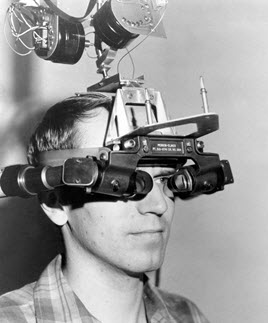
\includegraphics[width=0.4\textwidth]{photo1_sutehrland}
	\caption{Sutherland's Head Mounted Display \cite{photo1_Sutherland}.}
	\label{fig:sutherland_Display}
\end{figure} 


\par In 1976, this innovative technology led Ivan Sutherland to create the first head mounted display that was connected to a virtual environment, seen in figure \ref{fig:sutherland_Display}. Similar to modern virtual hardware, Sutherland's display consisted of glasses with two small screens that created the illusion of three-dimensional vision. The display allows the user to change what they observed by moving their head. This technology required a complex motion tracking system attached to the ceiling. Although groundbreaking, Sutherland's device did not let the user interact with the virtual environment.

\par Even though the technology did not exist, Sutherland had a vision of an ultimate stage of VR development, and how it could be achieved. A challenge was set that has motivated the progress of VR ever since: 

\begin{quote}
	The screen is a window through which ones sees a virtual world. The challenge is to make that world look real, act real, sound real, and feel real  \cite{gobbetti}. 
\end{quote}

The challenge was accepted by a man named Myron Kreuger, who coined the term artificial reality around 1970. Krueger created the first virtual system that allowed a user to interact with objects in a virtual environment. Through various sensors, the user's activities were monitored, allowing feedback within the program. Virtual object interaction was a major advancement towards completing Sutherland's challenge and inspired many new technologies to follow suit.  

Since Kreuger, VR development has continued to grow and become more popular, seeing many new innovations. VR in the media played a huge part in the popularization of the term. Movies like Tron and the Matrix imagined virtual worlds so advanced that distinguishing them from reality became nearly impossible. Though VR technology advancements continued through the 70's and 80's, Sutherland's challenge had only been achieved through film and imagination. 
In the 1990's, the Cave Automatic Virtual Environment, or CAVE was created.

\begin{figure}[h]
	\centering
	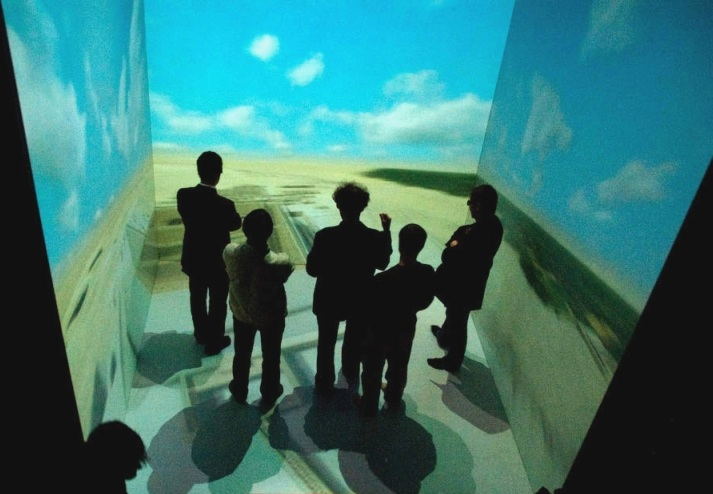
\includegraphics[width=.55\textwidth]{photo16_cave}
	\caption{CAVE: 4 Screens With 4 Stereoscopic Projectors \cite{CAVE}.}
	\label{fig:cave}
\end{figure}


CAVE was a large room full of screens that displayed a virtual environment, taking a different approach to VR hardware \cite{mihelj_apps}. One could also wear special glasses that made objects seem more three-dimensional in the eyes of the user. In addition, special sensors and surround sound were also used to promote immersion. Something else unique about this hardware was that and multiple users could fit in a Cave, enabling collaboration within the virtual environment. In just 60 years, the concept of VR was born and turned into a reality. Today, perfectly immersive virtual worlds have yet to be achieved, but the advancements and uses of VR have reached heights previously thought impossible. 



\section{Applications}\label{Apps}

Virtual Reality enables people's imaginations to run wild. Although the age of consumer VR is just beginning, the current range of applications is tremendous. One of the most prevalent areas of VR is within the gaming industry. Virtual reality gives gaming the potential for a user to become immersed in the virtual world. In lieu of a keyboard and mouse, haptic hardware gives users the opportunity to interact with virtual objects on a whole different level, changing immersive gaming as we know it. The potential for deep immersion, virtual presence and the production value  VR has to offer as an industry is driving developers and manufacturers to take part in the emerging field \cite{parisi}.   

 \begin{figure}[h]
	\centering
	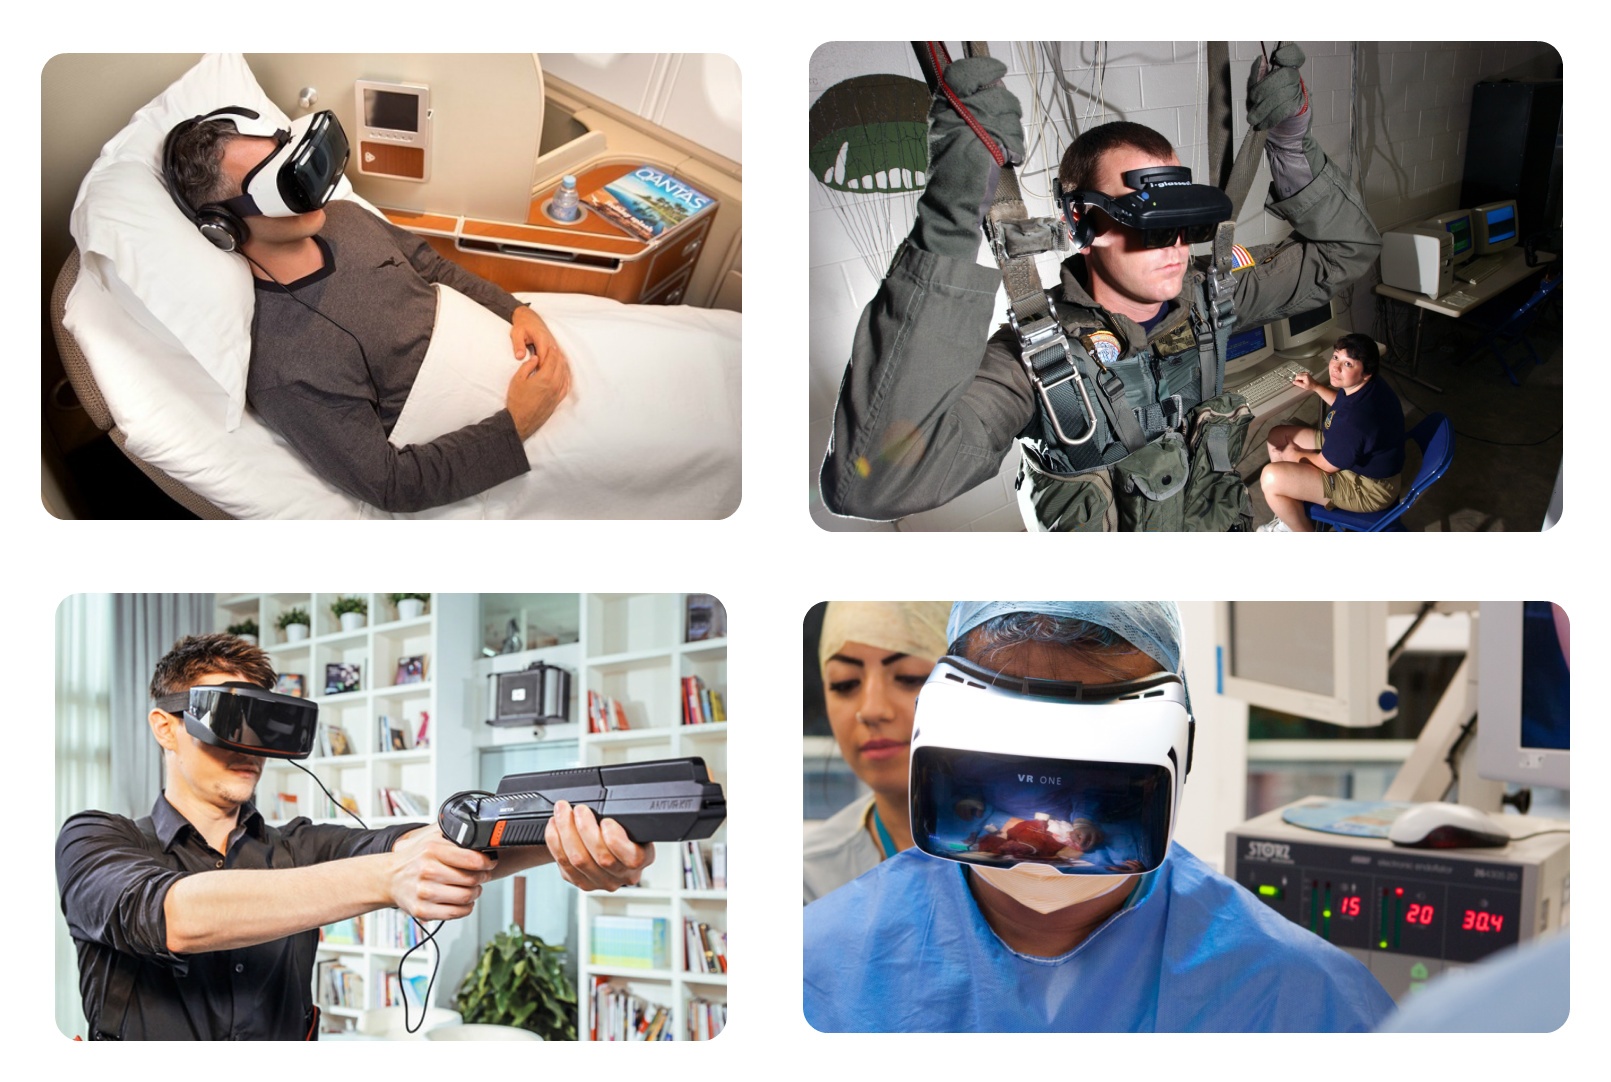
\includegraphics[width=.6\textwidth]{photo8_applications}
	\caption{VR Medical Applications \cite{applications}.}
	\label{fig:applications}
\end{figure}

However, new haptic and visual technology are not just being used for entertainment. Virtual reality is already successfully being used in many other applications, some of which are seen in Figure \ref{fig:applications}. The creation of immersive 3D virtual environments has enabled VR to be used in military training, medical training, and all types of design and engineering.These examples are just the beginning. The potential for VR in our modern day society is endless, ranging from interactive tourism to psychotherapy. With more and more foreseeable applications in todays society, the demand and technological innovations will just continue to increase, making VR development even more prevalent and expansive. 

\section{Virtual Presence}\label{presence}

VR is a unique form of media quite unlike other medias such as books or movies and should be dealt with as such. To acquire virtual presence while reading a book, the reader must leave their current reality behind to enter the reality of the text \cite{mihelj_apps}. VR requires the opposite. With VR, the user is placed into an environment and is meant to perceive and respond to it as though it were real. Virtual presence is the feeling of actually existing within a a virtual environment. In the words of Albert Einstein, reality is merely an illusion, albeit a very persistent one. Creating a successful virtual environment requires the creation of a successful illusion.  An effective illusion is made possible through a strong virtual presence. Virtual presence is achieved mentally, physically, or by a combination of the two. 

\subsection{Physical Presence}\label{physical presence}

Physical presence is an essential part of VR and takes place when the user's body physically enters the simulation or environment. It is truly what sets VR apart from other media.  In response to the users actions, select stimuli are presented to the user that affect their perception of the environment. Specifically, virtual environments are described through sight, sound and touch. These sensory perceptions define user interaction in a virtual world and are described in greater detail in the following section. 
	
\par The goal to obtaining optimal virtual presence is reducing as much real world stimuli as possible.
When immersed in the environment, virtual stimuli work to replace the user's exposure to real stimuli, decreasing mental and physical presence in the real world. Physical and mental presence go hand in hand. If physical stimuli are tricked to make you think you are present in a different environment, your mental presence in that environment also increases. 
	
	
	\begin{figure}[h]
		\centering
		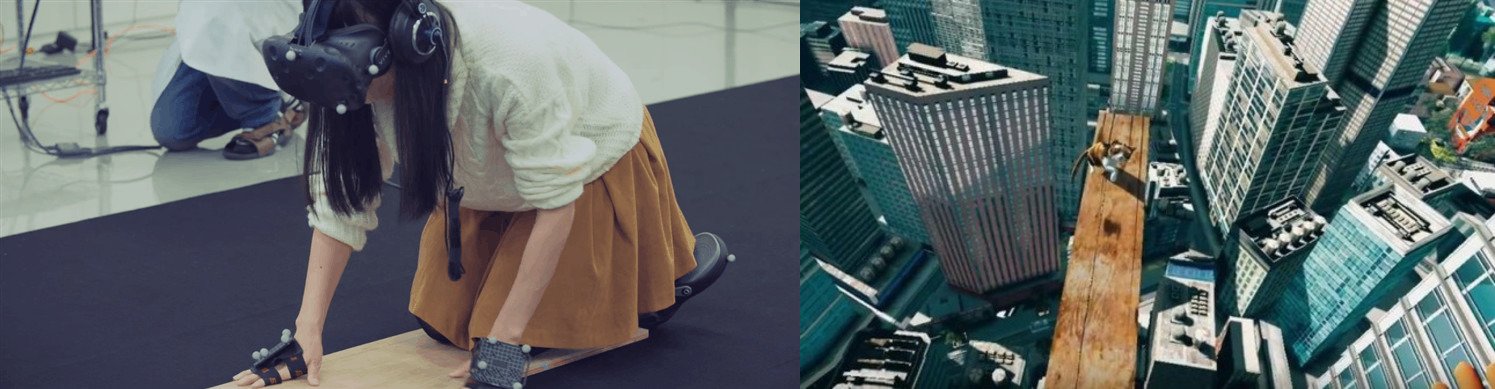
\includegraphics[width=\textwidth]{savecat}
		\caption{Virtual Presence: Fear of heights - save the cat or die trying \cite{matulef}.}

		\label{fig:savecat}
	\end{figure}
	
	
\subsection{Mental Presence}\label{mental presence}
	
	
It is possible for a user to be so immersed in a virtual world that it becomes their reality. Figure \ref{fig:savecat} is an example of a game made by Bandai Namco that challenges the user to save a cat from a wooden plank suspended thousands of feet in the air. This game creates mental presence by provoking very real fear among its users, so real that many are not able to save the cat successfully. Mental presence is the non-physical state of engagement felt after entering a virtual world. Achieving and maintaining mental presence is a very delicate and complicated process. There are many factors that affect mental presence. This also means many factors can destroy an immersive process. For example, a sense of virtual realism can be destroyed by small environmental defects because they distract the user from perceiving the scene as legitimate. The level of mental  presence is affected by the virtual scenario, the quality of realism, the number of senses stimulated, and the delay between the users actions and its effect on the virtual world. Mental presence within a virtual reality is difficult to achieve because all of these factors must be taken into account. In order to  successfully obtain virtual presence, a minimum level of physical and mental presence is key.  

\section{Conclusion}\label{intro_conclusion}

Virtual reality has a rich history and a bright future. The technological advances VR has made in the past 60 years and the current range of applications show the incredible potential of the growing field. For a virtual environment to be immersive, both the mind and body must believe they left their world behind and entered a new one. Physical and mental presence are crucial for a virtual space to be successful. The next chapter dives into the human sensory system and why it must be understood in order to model immersive environments that successfully capture the physical and mental presence of a user. 


%!TEX root = ../username.tex


\chapter{Human Sensory Perception: Biological and Cognitive}\label{Perception}

 VR is created through an exchange of information between the user and the virtual environment. For VR to be realistic, there must be a certain degree of responsiveness to a user's actions or inputs. Interaction within a virtual environment can be broken down into three categories: manipulation, navigation, and communication. 
 Manipulation allows the user to interact and make modifications to the virtual world and the objects within it. This interaction increases mental presence within an environment by promoting creativity and expression. Navigation permits the user to maneuver through the world, giving an illusion of depth within an environment. Effective navigation techniques require the user to create a mental picture of the environment, inherently promoting mental presence. Communication enables interaction between users and intermediaries in a virtual environment. Having multiple users in an environment enables an exchange of information and experiences \cite{mihelj_apps}.

%\section{Human Interaction} \label{interaction}


%%%%%%%%%%%%%%%%%%%	
%				  %	
%      SIGHT      %
%				  %
%%%%%%%%%%%%%%%%%%%

\section{Human Visual System} \label{sight}


Visual perception is considered to be the most dominant sense. Human cognition is oriented around vision, demonstrated by the fact that the visual system is given precedence over the other senses when conflicting inputs are present \cite{gobbetti}. A large area of the brain is dedicated to interpreting how we process the information gained from visible light. Because human behavior is so visually oriented, visual perception is given the utmost priority during any virtual experience. Due to the significance of visual perception, the frequency at which intermittent stimulus appear to be steady and in constant motion, or the critical fusion frequency, is an integral aspect of the visual system. Light perception, color perception, depth perception, field-of-view, and critical fusion frequency are vital components of the visual system and are discussed briefly in the next subsections with an emphasis on depth perception. 

\subsection{Light Perception} \label{sight_perception} 

It is important to understand exactly how light perception works. Figure \ref{fig:humaneye} is useful for the following description. First, visible light from the environment enters the eye through the transparent cornea. The light intensity is controlled via the pupil, which can limit the amount of light entering the eye by dilating or contracting. Behind the pupil is the lens, whose job it is to focus light on the retina. The lens, which is attached and controlled by the ciliary muscle, is able to contract in order to change its thickness. Changing the thickness of the lens enables objects at different distances from the eye to be clearly seen \cite{mihelj_apps}. 
%\cite{VR Tech and Apps}.

\begin{figure}[h]
	\centering
	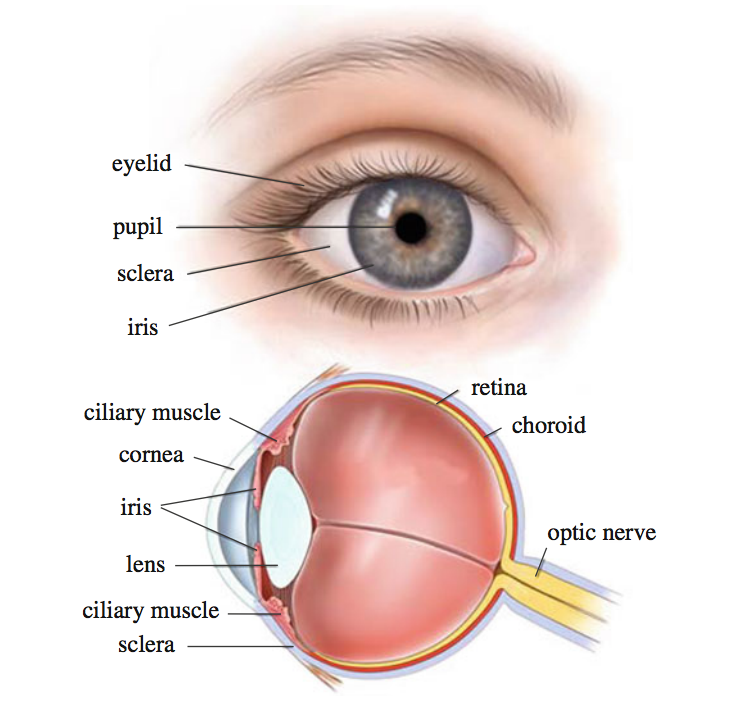
\includegraphics[width=.5\textwidth]{humanEye}
	%cite VR tech and Apps
	\caption{The human eye \cite{mihelj_apps}.}
	\label{fig:humaneye}
\end{figure}

\par The retina contains photoreceptors that are specialized light-sensing nerve endings. Photoreceptors can be divided into cones and rods. Cones sense colors, react quickly to light intensity changes, and are less sensitive to light. Rods do not sense color, are more sensitive to light, and allow sight during conditions with low levels of light. The light picked up by these receptors is then converted into an electrochemical signal that travels across the optic nerve. The optic nerve connects to the visual cortex in the brain, which turns the incoming signals into the images we then see \cite{mihelj_apps}.

\subsection{Color Perception} \label{color_perception} 

Using the cones in the retina, the human eye is able to sense varying levels of color. There are three types of cones in the eye that are able to pick up different wavelengths of light. The tiny wavelengths of visible light that humans can "see" range from 380 to 700 billionths of a meter, expressed as nanometers or nm. The first cone type senses red light (564-580nm), the second type senses green light (534-545nm), and the third type of cone picks up blue light (420-440nm) \cite{mihelj_apps}. The shorter wavelengths are known as ultraviolet light and the longer wavelengths are called infrared light.


\begin{figure}[h]
	\centering
	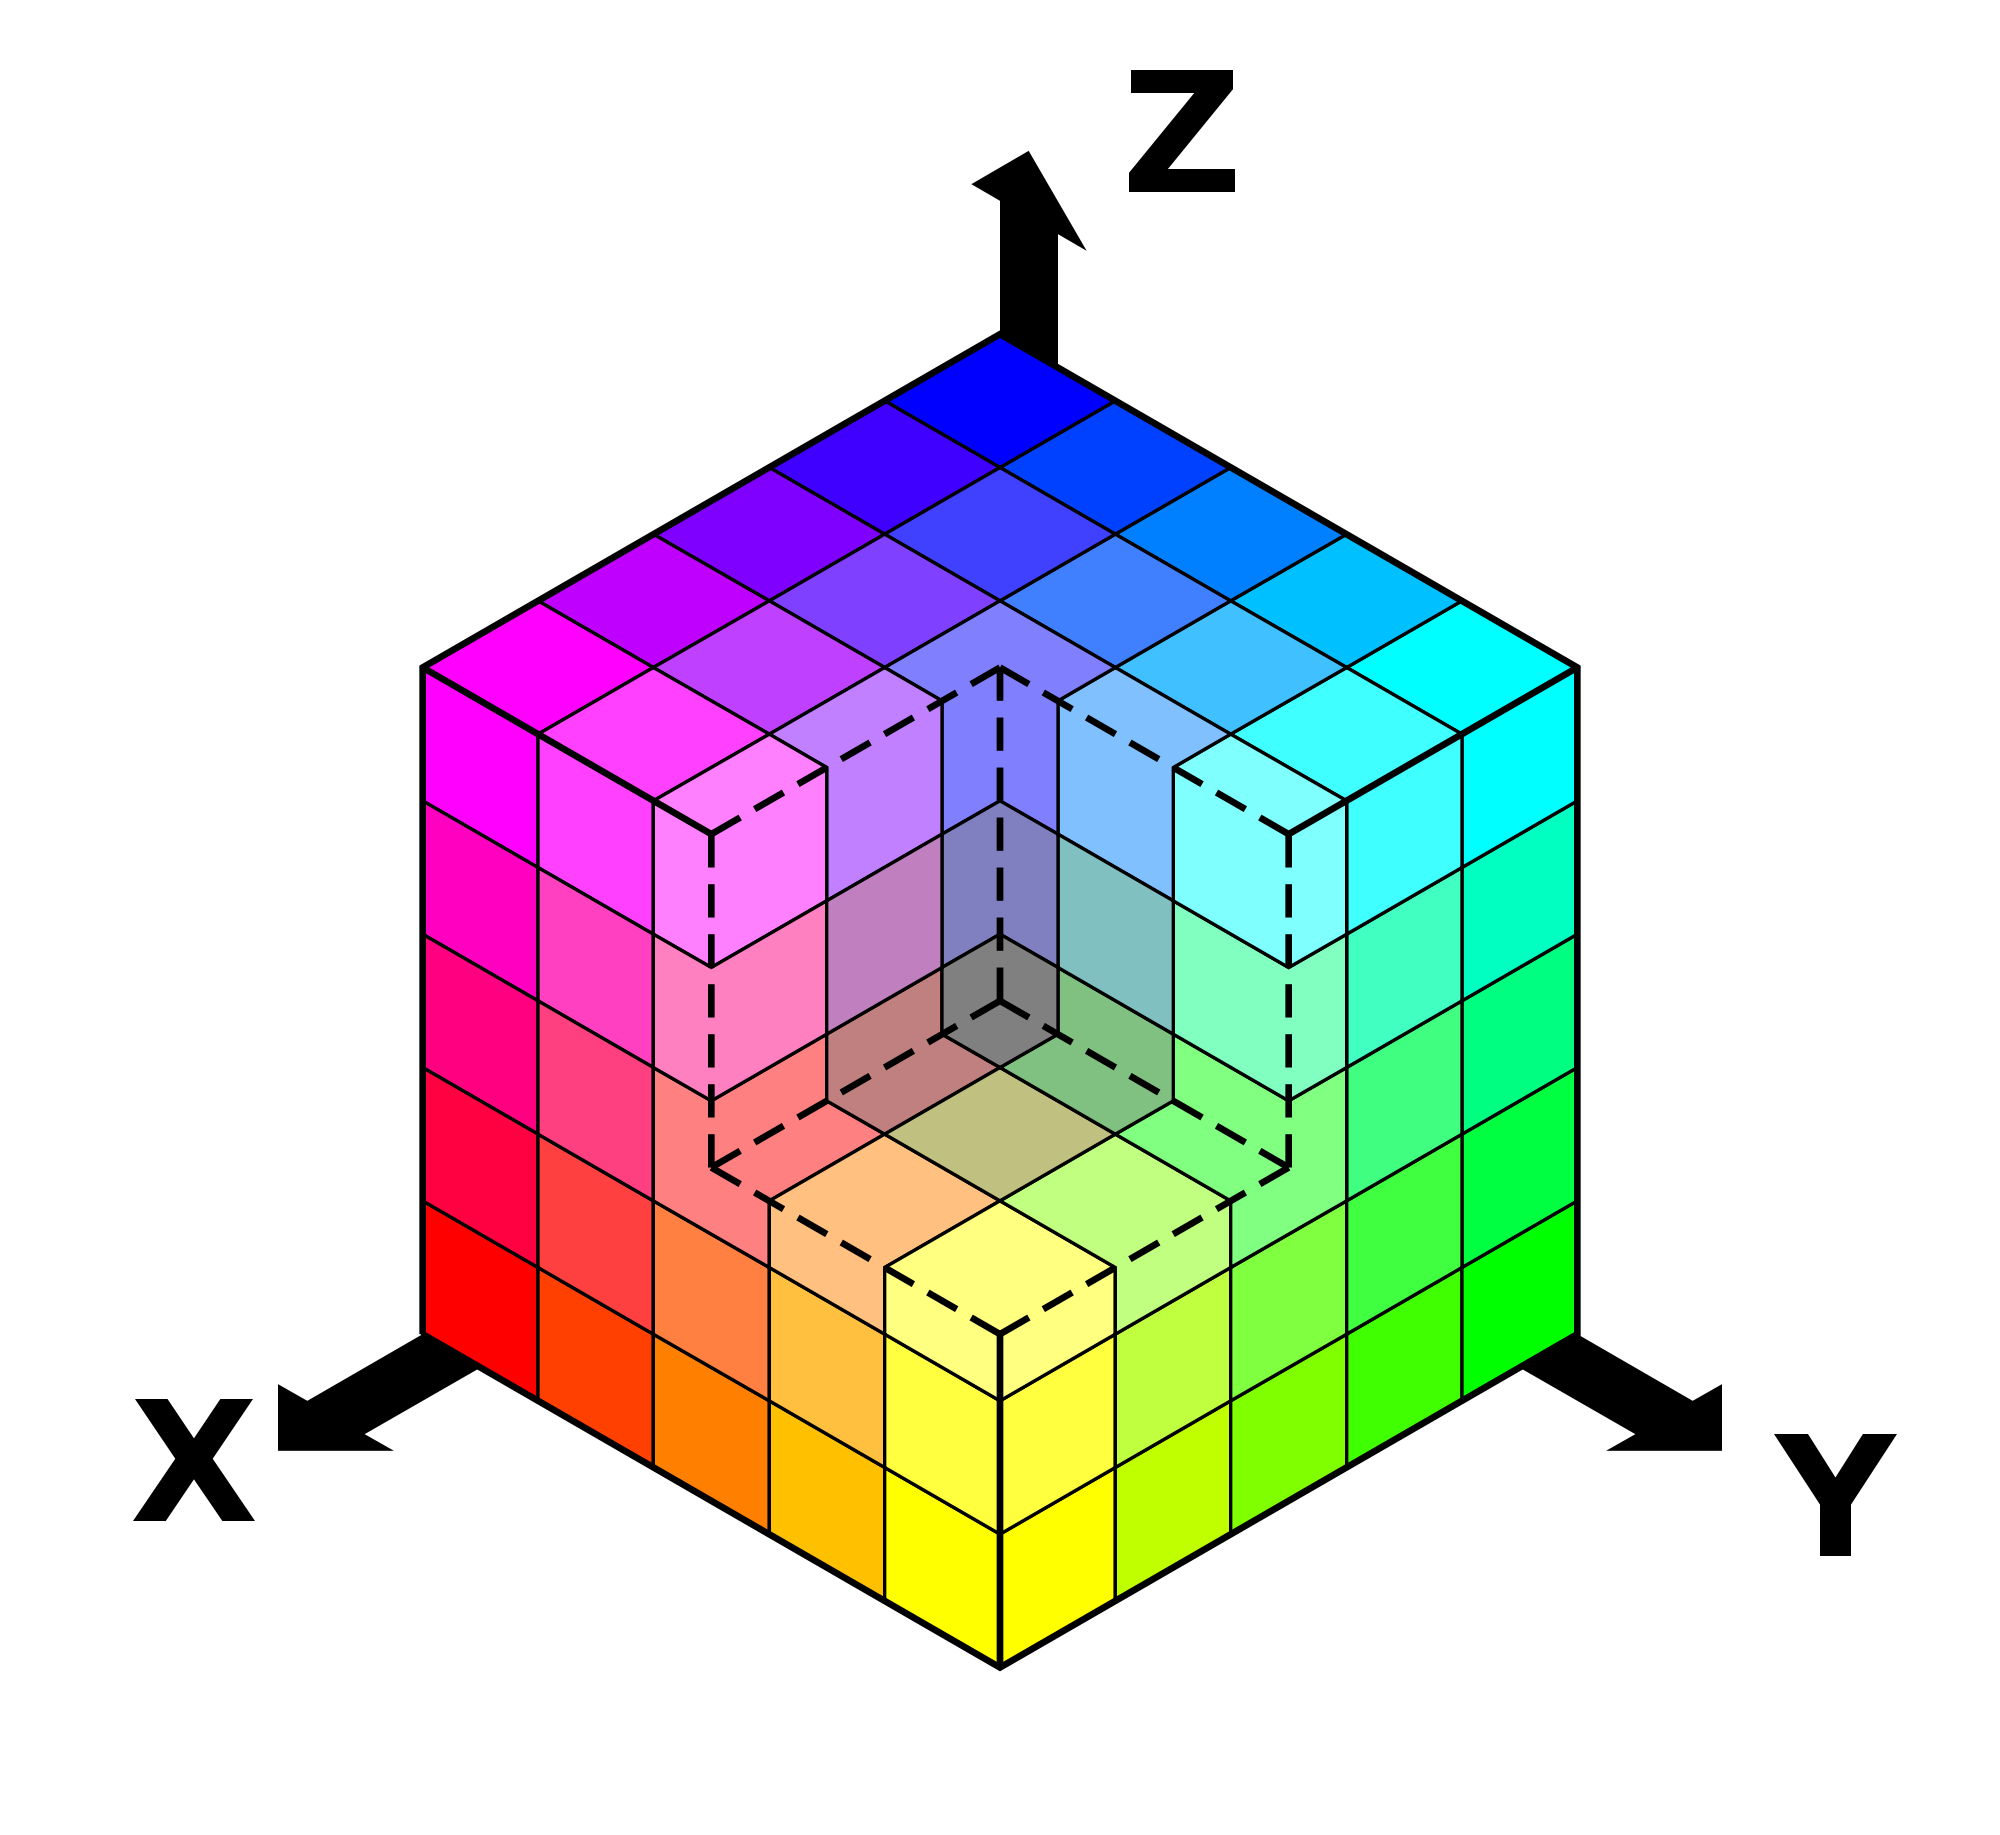
\includegraphics[width=.5\textwidth]{RGB_Model}
	\caption{Representation of the RGB Model \cite{_color}.}
	\label{fig:RGB_Model}
\end{figure}

\par In virtual environments, modeling is usually done using these primary colors in order to match the three types of cones in the human eye. The most frequently used model is the RGB model, representing red, green and blue colors. This model, seen in Figure \ref{fig:RGB_Model} allows any combination of colors to be created simply by combining a mixture of the three primary colors detectable by the human eye. 



\subsection{Depth Perception} \label{depth_perception} 


One of the most important functions of the human visual system is its ability to determine the distance to particular objects. This concept, known as depth perception, is extremely important in virtual realty. Since virtual displays do not always incorporate depth into a scene, VR designers must understand depth cues in order to fool the human senses and and create a virtual illusion of depth. The human mechanisms for determining depth can be divided into monoscopic and stereoscopic depth cues.

\par Monoscopic depth cues are received by just one eye and exist in two-dimensional images. From 
%\cite{vr tech and apps: pg. 99}
\cite{mihelj_apps}, Monoscopic depth cues include those listed below and several are depicted in Figure \ref{fig:depth}. 

\begin{figure}[h]
	\centering
	\includegraphics[width=.6\textwidth]{DepthPerceptionCues}
	\caption{Depth perception cues \cite{depth}\cite{texture}\cite{filippini}\cite{LinearPerspective}.}
	\label{fig:depth}
\end{figure}

\begin{enumerate}
	\item \textit{Occlusions:} Objects in the foreground obstruct those in the background.
	\item \textit{Shading:} Shading indicates the relative size of different objects and offers an estimate of their shape.
	\item \textit{Size:} Size allows comparisons between objects of different sizes, allowing us to gauge their relative distance.
	\item \textit{Linear Perspective:} Parallel lines appear to converge at a point as they recede into the distance. This can be used to determine the relative size, shape or position of an object by imagining or drawing these lines.
	\item \textit{Surface Texture:} Since the human eye cannot pick up sutle detail at great distances, objects further away have a less sharply defined texture than those that are closer.
	\item \textit{Accommodation:}  Accommodation is the dilation or contraction of the lens  in order to keep an object in focus as its distance from the eye varies. This process allows the brain to estimate the distance to an object based on the lens thickness.
	\item \textit{Parallax:} When the viewer is in motion, objects further away appear to move less in the field of view than objects that are closer to the view. 
	\item \textit{Movement of the view object:} When objects move further away from the viewer, they appear to grow smaller. When objects move closer to the viewer, they appear to become larger. This information allows the brain to estimate how long an approaching object has before it collides with the viewer.
\end{enumerate}





\par On the other hand, stereoscopic depth cues combine the information gathered from both eyes. Stereoscopic viewing is the primary way the visual system perceives depth. As objects become further than 30 meters away, many of the geometric benefits of stereopsis fade \cite{gobbetti}. This makes stereoscopic depth cues extremely effective for observing objects that are at closer distances. From \cite{mihelj_apps}, the stereoscopic depth cues are the following:


\begin{enumerate}
	\item \textit{Convergence:} The process where the eye turns inward toward an object in order to focus on that object, pictured in Figure \ref{fig:convergence}. This process allows the brain to judge the perceived depth of that object. 


	\item \textit{Stereopsis:} A process that allows depth to be estimated based on the difference between what the left and right eye perceive. 
\end{enumerate}


\begin{figure}[h]
	\centering
	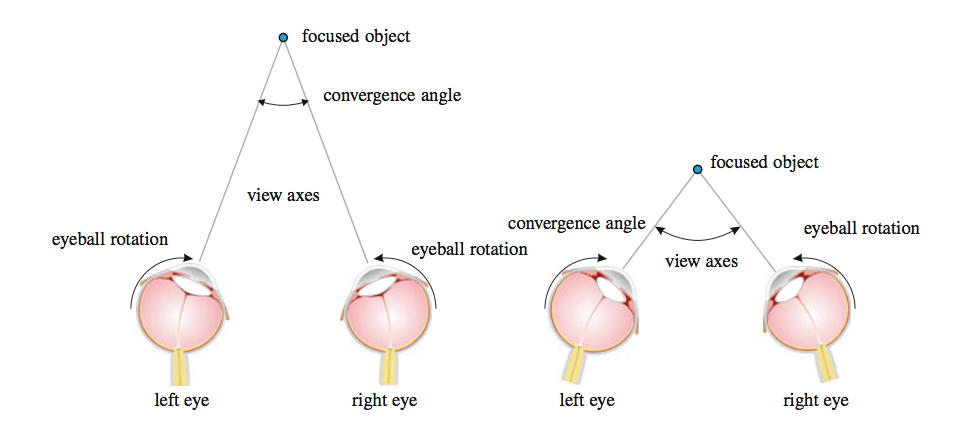
\includegraphics[width=.7\textwidth]{convergence}
	\caption{The Process of Convergence \cite{mihelj_apps}.}
	\label{fig:convergence}
\end{figure}

% cite haptics for VR and tele : pg 8
If there are conflicts between different depth cues, stereopsis takes precedence over all others \cite{mihelj_haptics}. A virtual environment can be designed using any of these cues to create a perceived feeling of depth. The more cues that are incorporated into a scene, the more realistic the illusion of depth becomes.


\subsection{Field Of View And Critical Fusion Frequency} \label{fov_criticalfusionfrequancy} 

Field-of-view, and critical fusion frequency also have an important role on the visual experience of immersive virtual scenes. The complete field of view for human eyes is around 180 degrees horizontally, and over 120 degrees vertically. Therefore, in order to create a successful optical illusion, the field of view should be 90 to 110 degrees \cite{gobbetti}. 
 
 
 \begin{figure}[h]
 	\centering
 	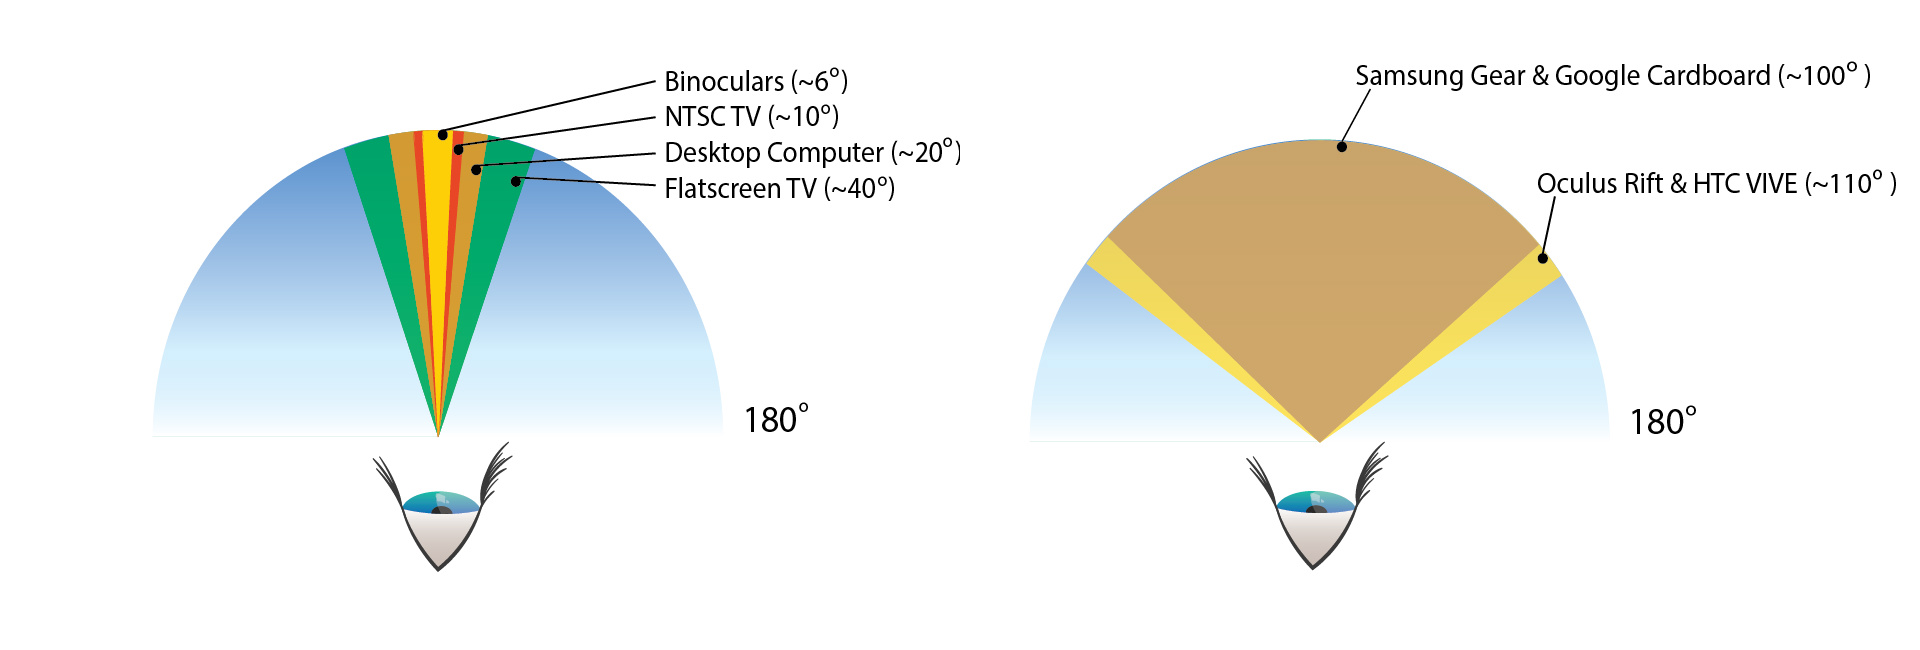
\includegraphics[width=.85\textwidth]{fov}
 	\caption{Field of view comparisons \cite{markiewicz_6_2015}.}
 	\label{fig:fov}	
 \end{figure}

 Different head mounted displays offer varying fields of views. As seen in Figure \ref{fig:fov}, the HTC Vive offers 110 degrees, an optimal field of view for VR applications. The critical fusion frequency is the rate that humans can distinguish between successive visual stimuli. For example, when the frequency is too small, object movement is choppy and no longer fluid. In computer graphics, a rate below 30-60 Hz results in this effect. 
 % do i remove this since it was already defined? or move it?
  

 \par  A narrow field of view and low frame rates in VR cause distraction and remind the user of their presence in a virtual setting. Visual displays, like the VIVE, require stereoscopic vision and must deliver stimuli of acceptable resolution, high-quality motion representations and satisfactory levels of brightness \cite{gobbetti}. Given the significance of the visual system, visual displays have become the most important piece of VR hardware. However, head mounted displays are not always enough. Virtual environments should not only engage a user's visual and auditory senses, but also offer user interaction mechanisms. Haptic hardware is able to create interactive connections between the user and their environment, an aspect absolutely critical in achieving an immersive application.
 
 \begin{figure}[h]
 	\centering
 	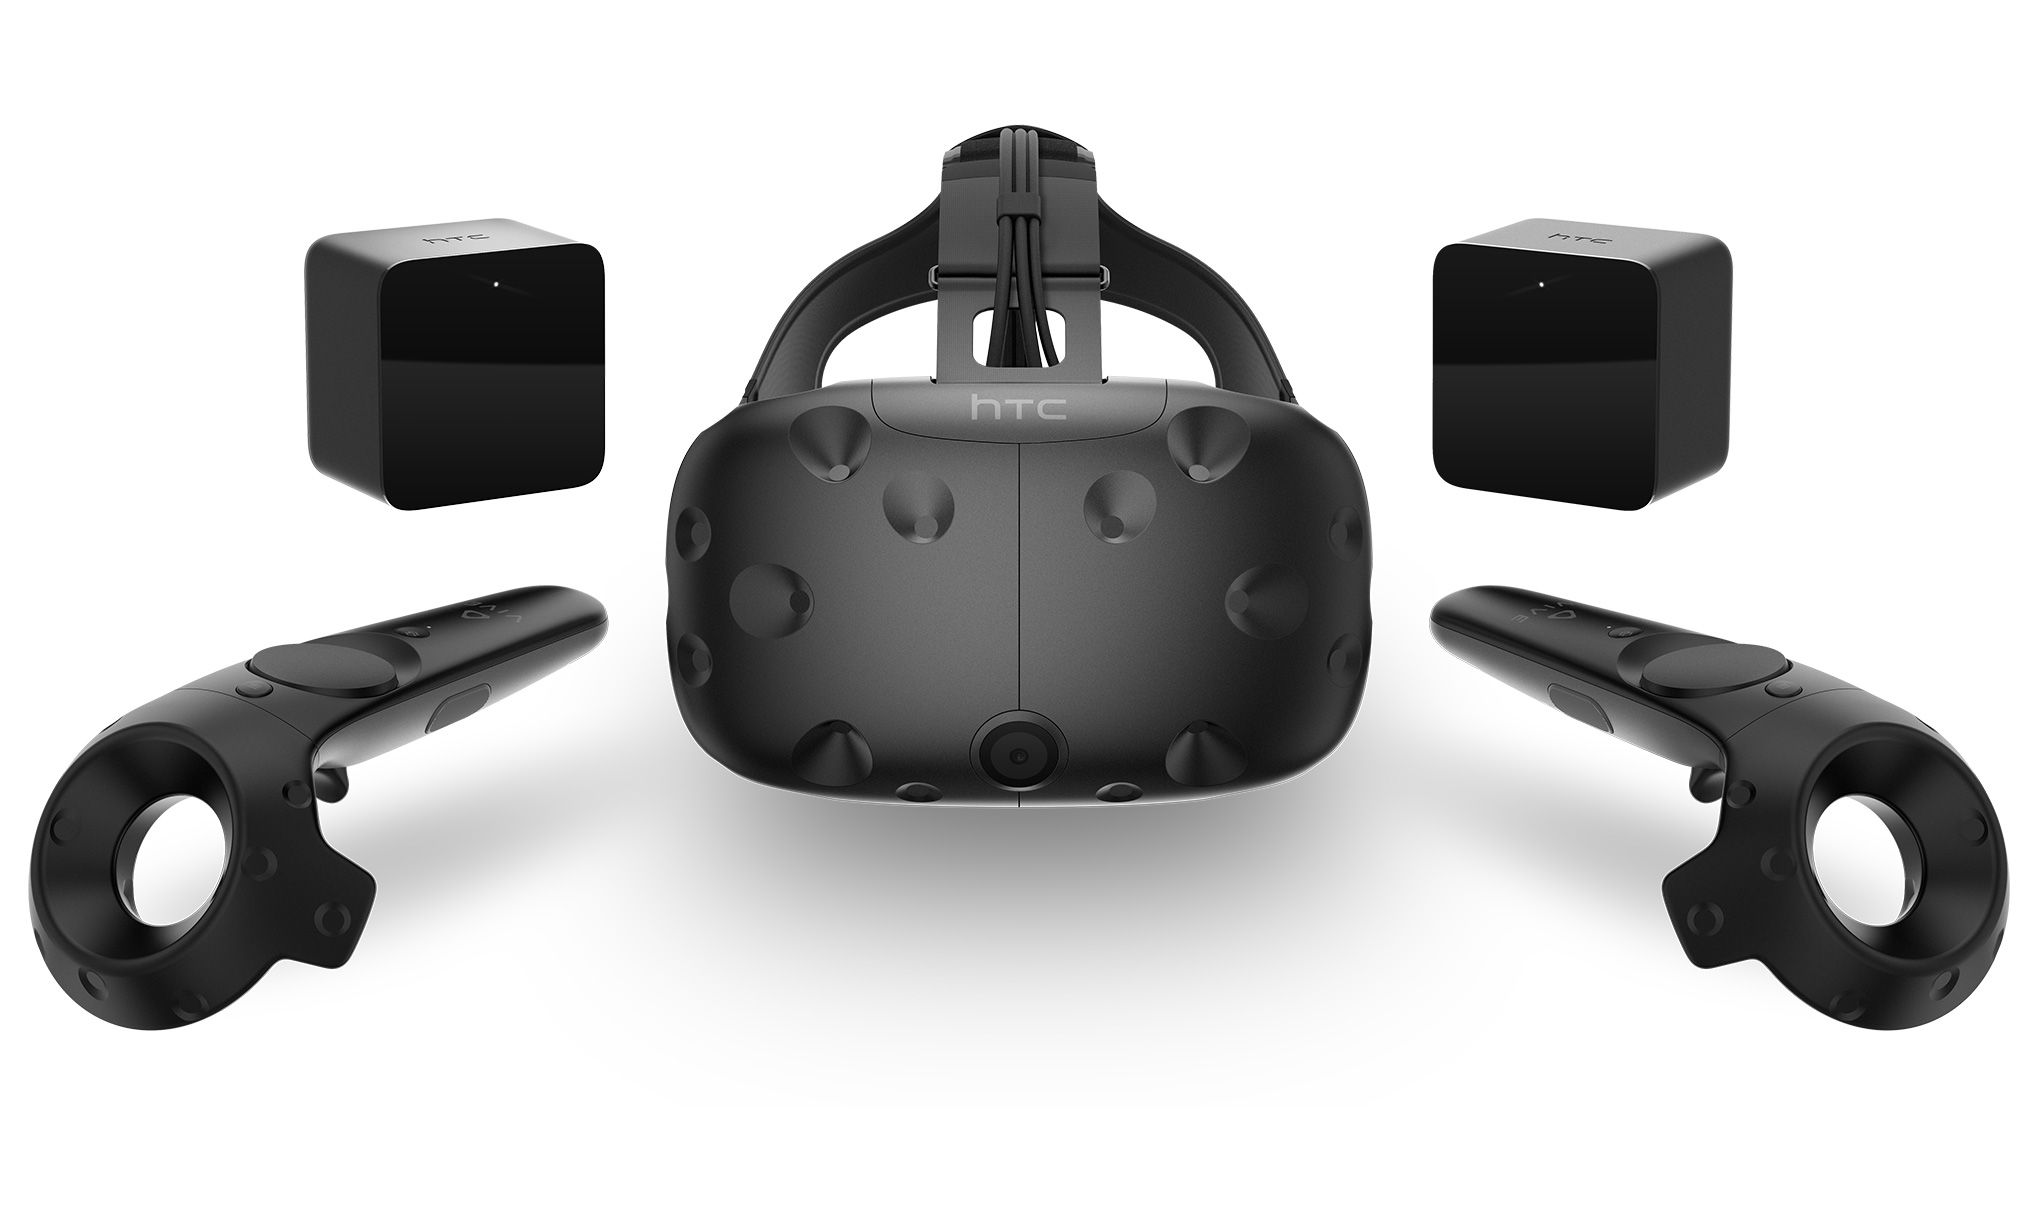
\includegraphics[width=.6\textwidth]{htc_vive}
 	\caption{HTC Vive with hardware - including haptic controllers \cite{walton_psvr_2016}.}
 	\label{fig:vive}
 \end{figure}


 
 
 %%%%%%%%%%%%%%%%%%%	
 %				   %	
 %      TOUCH      %
 %				   %
 %%%%%%%%%%%%%%%%%%%
 

\section{Human Haptic System} \label{touch}

% + definition of haptics
% + haptic perception
% + haptic applications?
% + haptic representation in VR
% + haptic rendering in VR


% intro: definition of haptics

The word \textit{haptic} comes from the Greek verb \textit{hapto}, meaning \textit{to touch}. %cite hapticsfor VR pg 35
Haptic refers to the exploration and process of identifying objects through touch \cite{mihelj_haptics}. %cite haptics for VR pg.10
An effective VR system utilizes haptic devices to enable a user to interact with objects in a virtual environment through gestures. Figure \ref{fig:vive} shows the HTC Vive, an example of a commercially popular head tracking system that is also equipped with haptic controllers. A haptic device mimics tasks that would normally be performed in the real world, such as gathering information about an object and its properties. A haptic interface is a device that measures a position or contact force and displays that contact force or position to the user. To put it even more simply, a haptic interface receives motor commands from the user and displays haptic images back to the user \cite{mihelj_haptics}. The human hand allows a user to push, grasp, squeeze or hit objects. When transfered into a virtual space, being able to touch, feel and manipulate objects results in a level of immersion that is not possible without a haptic system. Haptic hardware in VR allows the user to perceive information about the virtual world, and the rules that govern it. Many new games use haptic hardware that allows the user to interact and manipulate objects in the virtual world. A game called Job Simulator, illustrated in Figure \ref{fig:job_simulator}, implements these strategies to allow the user to interact with objects as part of the storyline. The inability to have this level of interaction within an environment makes it impossible for a user to truly perceive a virtual world as real. 


\begin{figure}[h]
	\centering
	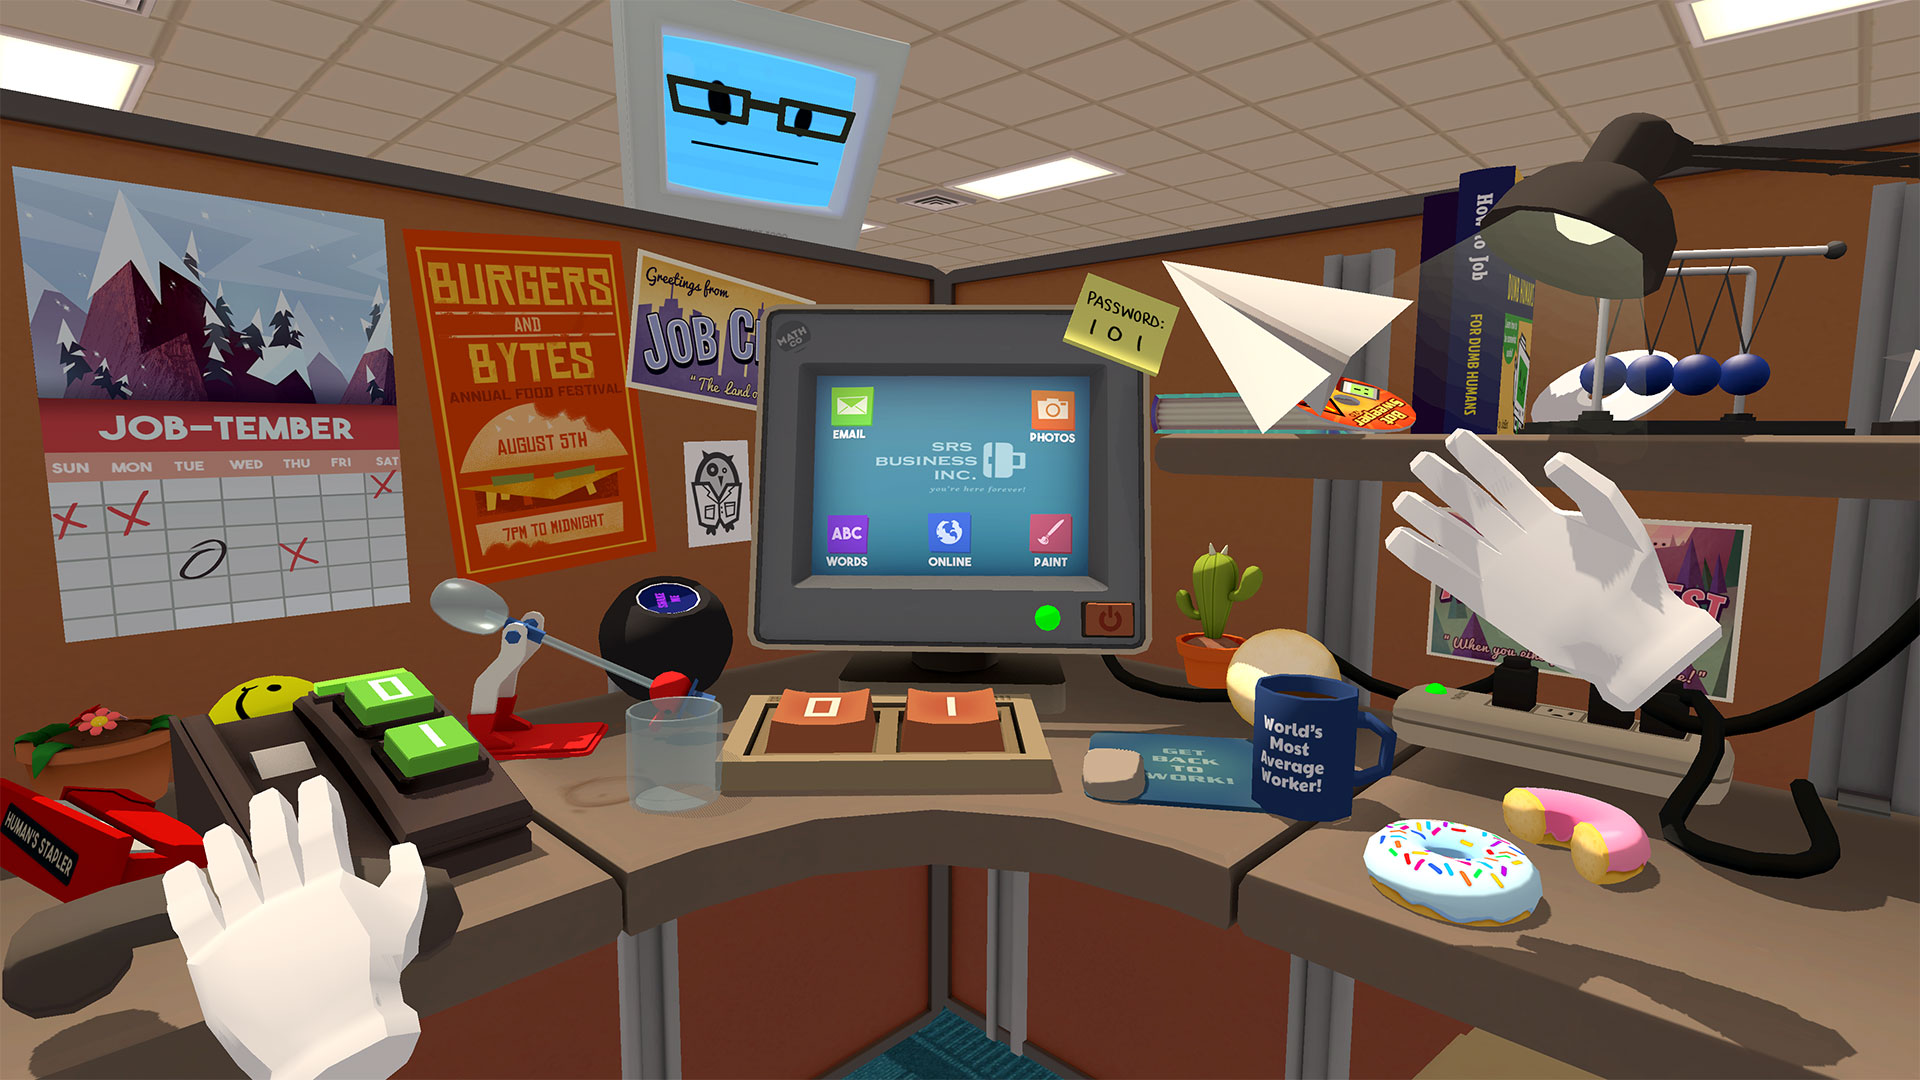
\includegraphics[width=.7\textwidth]{job_simulator}
	\caption{Job Simulator: An interactive game that uses haptic hardware and object manipulation as it's primary tool for creating an immersive experience \cite{jobSim}.}
	
	\label{fig:job_simulator}
\end{figure}

%  haptic perception (basics)
 \par Haptic perception is different from vision and sound because it provides the ability to sense and also act upon an environment. Through touch, different types of information can be gathered when manipulating objects in the environment. The human haptic system is divided into three subsystems made up of sensory capabilities, motor capabilities and cognitive capabilities. Sensory capabilities use kinesthetic and tactile senses to derive information about the environment through touch. In VR, sensory capabilities can be used to give the user cues and insight on the virtual world and its rules. Motor capabilities use the musculoskeletal system to gain information about and manipulate objects through interaction. Cognitive capabilities use the central nervous system to analyze information gathered from an environment and plan motor functions based on the objectives of the tasks. When designing haptic interfaces, understanding the haptic system is imperative.



%%%%%%%% this seems repetitive %%%%%%%%
%The information gathered can be characterized as either tactile or proprioceptive \cite{gobbetti}. Tactile information is gathered from an initial touch of an object. This provides knowledge of the shape and the texture of the object. Applying extended force to an object provides proprioceptive information of the object's weight, forces acting upon the object and surface compliance \cite{gobbetti}. Combining tactile and proprioceptive cues allows the user to feel present and engaged within a virtual setting.
%%%%%%%% This also seems reptitive %%%%%%%%
%A haptic experience is based on tactile and kinesthetic senses. Tactile senses provide information based on the stimuli on the surface of the body. Kinesthetic senses give information about the pose and movement of the body.



\subsection{Sensory System} \label{tactile_kinesthetic}

 % explain active verse inactive movement...?
 \par Sensory information can be broken further into subclasses consisting of tactile and kinesthetic information. Tactile sensors transmit information to the brain about an object when initial contact is made. This information is gathered by low-threshhold mechanoreceptors  in the skin such as a fingertip \cite{mihelj_haptics}. When the hand is stationary and comes into contact with an object, tactile sensors are the ones to transmit information concerning that object. The type of information gathered by tactile sensors can range from the fine texture, size, softness, slipperiness and temperature of an object. On the other hand, kinesthetic information conveys the position, movement and forces acting on a limb \cite{mihelj_haptics}. When an arm or other limb is active in free space, this kinesthetic information gives insight regarding the natural shape, compliance and stiffness of surrounding objects. During any active task, sensory information is simultaneously gathered from both types of sensors, giving the brain constant feedback.
 
 \subsubsection{Kinesthetic Perception} \label{tactile_kinesthetic}
 
 The Kinesthetic system is primarily used to acquire information about the forces generated by certain muscles, and the resulting movement of limbs. However, kinesthetics also refers to the perception of force, an aspect extremely relevant in the topic of haptic interaction systems within virtual reality. Mechanoreceptors provide information to the central nervous system about static muscle length, muscle contraction velocity, and forces generated by muscles \cite{mihelj_haptics}. Other sensory information regarding the change of limb position are acquired from receptors in the joints and skin. The receptors in the skin play an important role in tactile exploration and interpreting the position and movement of the arms. This subsection gives an overview of the kinesthetic receptors, specifically mechanoreceptors, which are responsible for the perception of movement, force, and the position of limbs.
 
 \par  Mechanoreceptors are found in muscle spindles and are classified as primary and secondary receptors. Seen in Figure \ref{fig:receptors}, muscle spindles, found in muscles, are .5-10 mm in length and made up of bundles of muscle fibers \cite{mihelj_haptics}. Muscle fibers are attached at both ends to muscle or tendon fibers and are responsible for generating muscle force. These spindles identify changes of tension and length within muscle fibers. The primary role of muscle spindles is to act as an automatic safety device for the muscles. When the muscle is overly stretched, the spindles respond by stimulating a muscle contraction in order to prevent the muscle from extending or stretching too far. These automatic muscle contractions, or reflexes, are important for controlling movement and balance.
 
 
 \begin{figure}[h]
 	\centering
 	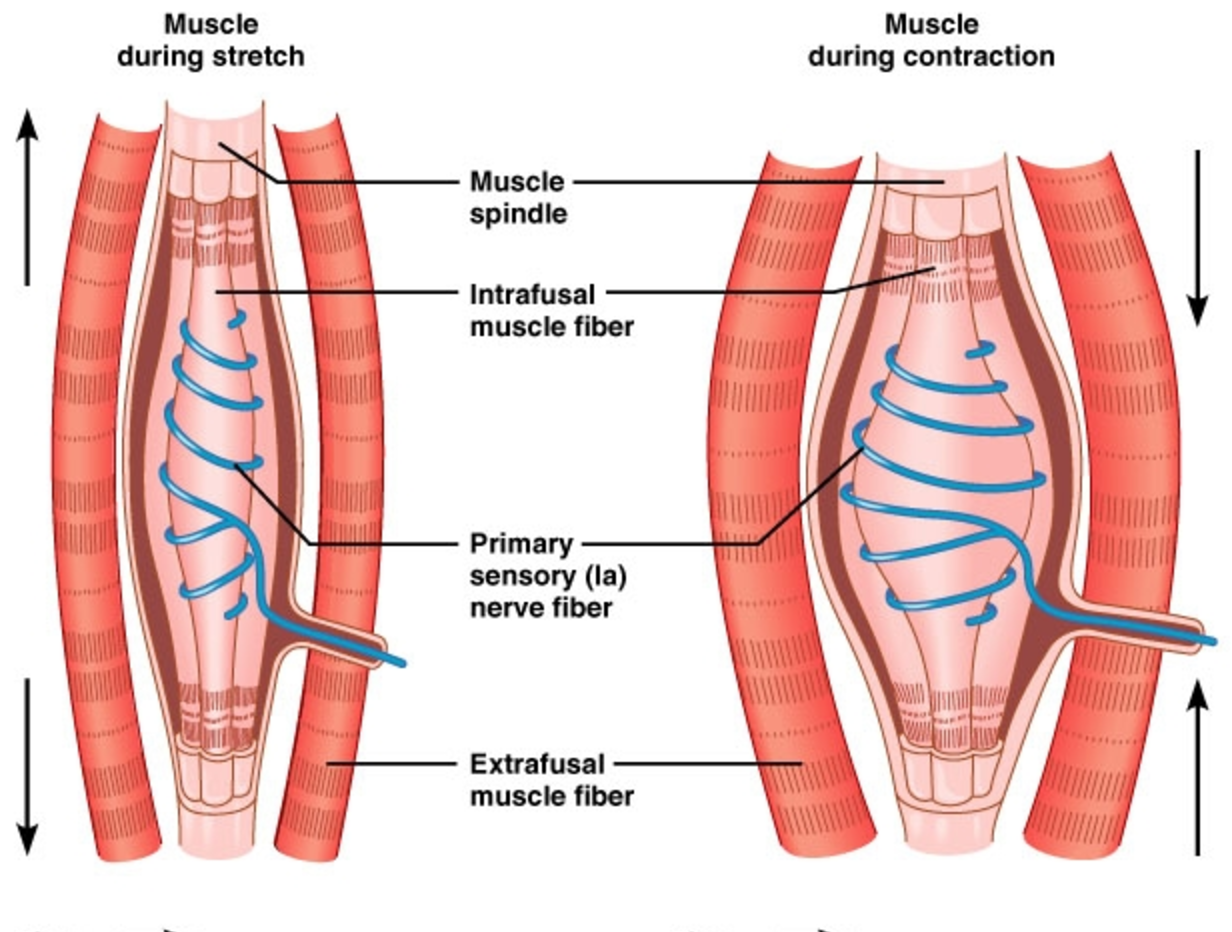
\includegraphics[width=.6\textwidth]{receptors}
 	\caption{Kinesthetic Receptors \cite{proprioception}.}
 	\label{fig:receptors}
 \end{figure}


 % Both primary and secondary spindle receptors respond to velocity, direction, movement, length and position of the lib. 
 

\par Each mechanoreceptor, primary and secondary, react to a change in muscle length and act accordingly. The primary spindle receptors dynamically respond to changes in muscle length by dealing with the velocity and acceleration aspects of movement. The job of the primary receptors is to modify the sensitivity of muscle spindles based on the muscle's length, contraction history, and current velocity of muscle contractions \cite{mihelj_haptics}. Primary receptors actively influence the velocity, direction and movement of a limb. In contrast, the secondary receptor's job is to output a constant static measurement of muscle length and position of the limb. Normally, an area with a high density of mechanoreceptors  means a highly functional tactile system. However, in a kinesthetic system, a higher density of receptors does not always mean better kinesthetic capabilities \cite{mihelj_haptics}. Instead, the size of the muscle, not the functionality, dictates the number of muscle spindles present. 


 
\begin{figure}[h]
	\centering
	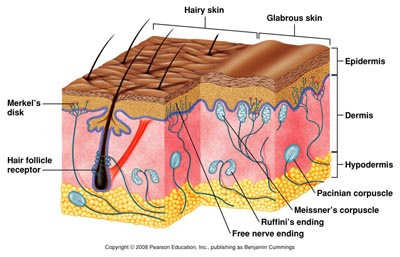
\includegraphics[width=.75\textwidth]{SkinReceptors}
	\caption{Ruffini Endings and Pacinian Corpuscles \cite{somatosensory}}
	%\cite: http://www.d.umn.edu/~jfitzake/Lectures/DMED/Somatosensation/Somatosensation/Receptors.html
	\label{fig:SkinReceptors}
\end{figure}


\par In addition to spindle receptors, there are other types of mechanoreceptors used within the human haptic system, displayed in Figure \ref{fig:SkinReceptors}.
Located where the tendon attaches to the bundle of muscle fibers, the Golgi tendon organ provides information about force exerted by muscles \cite{mihelj_haptics}. The Golgi tendon organ essentially serves as a safety mechanism by reducing muscle tension when the muscle is under an excessive load.  Ruffini endings and the Pacinian corpuscles are other mechanoreceptors found in the joints. The Ruffini endings sense angle and angular velocity of the joint movements. The Pacinian corpuscles are used to estimate joint acceleration and have a natural sensitivity that responds to both vibration and pressure \cite{mihelj_haptics}.


 \subsubsection{Tactile Perception}
 
 


 While the kinesthetic system works to acquire information regarding force and the movement of limbs, the tactile system defines and interprets sensations acquired through touch. The various and complex sensations generated during object interaction are made up of a few specific components. Roughness, lateral skin stretch, relative tangential movement and vibrations make up the sensations we receive when interacting with these objects \cite{mihelj_haptics}. The mechanoreceptors in the skin define the texture, shape, compliance and temperature that are all perceived through touch. Specifically, the Meissner's corpuscles, Pacinian corpuscles, Markel's disks and Ruffini corpuscles are the sensory organs in the skin that define a sensory experience. These sensory organs and their properties are displayed in Figure \ref{fig:Mechanoreceptors}
 
 
  \begin{figure}[h]
 	\centering
 	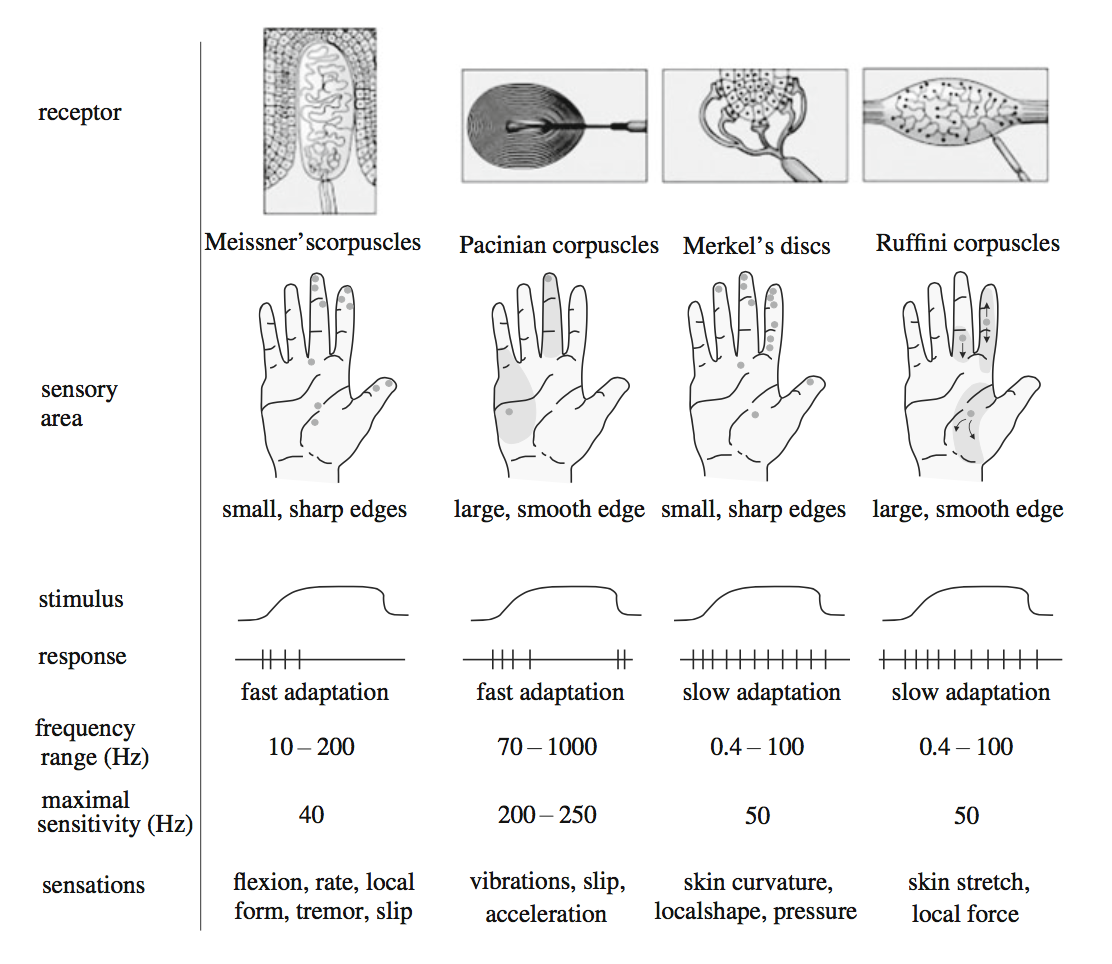
\includegraphics[width=.6\textwidth]{Mechanoreceptors}
 	\caption{Properties of Mechanoreceptors \cite{mihelj_haptics}.}
 	\label{fig:Mechanoreceptors}
 \end{figure}

 \par These four types of mechanoreceptors differ in size, receptive fields, rate of adaptation, location in the skin and physiological properties. Spatial resolution depends on where the receptors are located in the skin. Certain receptors have large receptive fields, which means they have a low spatial resolution. Others have small receptive fields, meaning they have a good spacial resolution. Each receptor also has a different rate of adaptation. When a receptor has fast adaptation, it detects short pules of sensory information. An example of fast adaptation is the initial contact with an object or the detection of a vibration. A slow speed of adaptation means the receptor detects a constant stimulus, like a constant pressure. Figure \ref{fig:Mechanoreceptors} displays the rate of adaptation of receptors in the skin. 
   


 \par Like color perception, the quality of a sensory experience is determined by a combination of responses from different receptors. Receptors are able to achieve a wide detection range for detecting vibrations and frequencies ranging from 0.4 to 1000Hz \cite{mihelj_haptics}. Frequencies over 500Hz are no longer felt as vibrations, but as having textural qualities. Given the properties of a tactile system, specifically the perception area, duration and frequencies are important for modeling interaction systems in virtual environments.


 
\subsection{Motor and Cognitive Systems} \label{motor_cognitive}
 
 
 \begin{figure}[h]
 	\centering
 	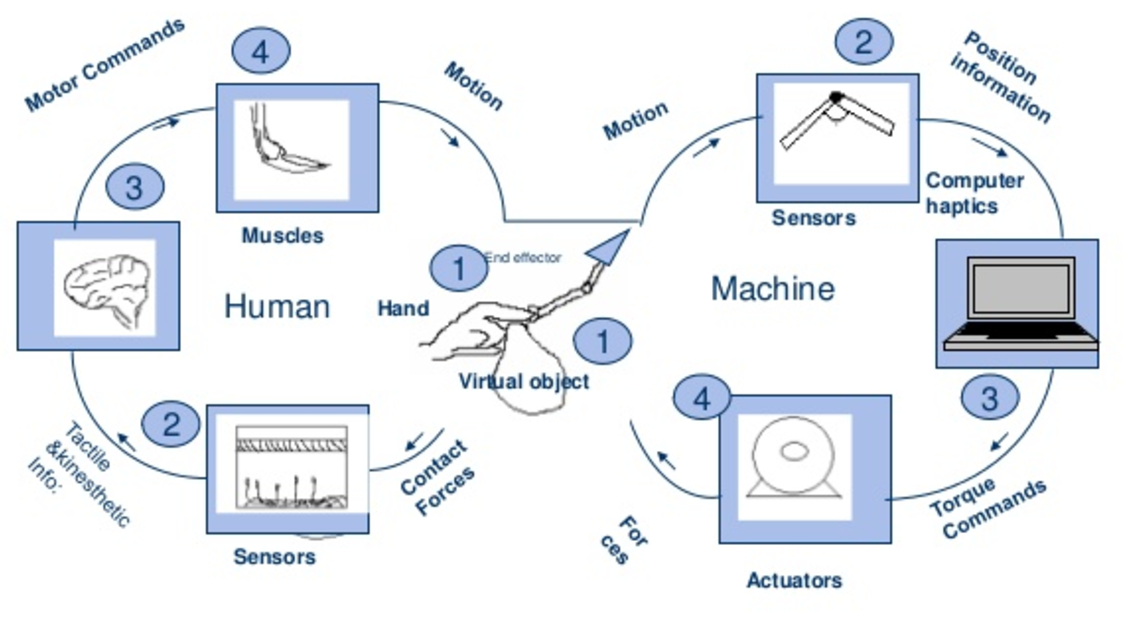
\includegraphics[width=.8\textwidth]{haptic_interaction}
 	\caption{Human-Machine Haptic Interaction \cite{ganesan}.}
 	\label{fig:haptic_loop}
 \end{figure}
 
 
  \par In addition to sensory capabilities, the motor system and the cognitive system make up the human haptic system. The motor system allows for active exploration of an environment and manipulation of objects within it.  The cognitive system associates action with perception \cite{mihelj_haptics}.  When designing a haptic experience in VR, understanding how these different haptic subsystems function and work enables a designer to build an interactive and realistic virtual environment. Figure \ref{fig:haptic_loop} displays how the haptic subsystems work together with a haptic hardware device to control the position of the hand and exert forces to simulate contact with a virtual object. The sensory, motor and cognitive systems all work together to construct a haptic experience. Both tactile and kinesthetic sensory information compose contact perception, while motor commands allow movement and navigation through an environment based on the cognitive objectives \cite{mihelj_haptics}. The more haptic subsystems used to define a virtual experience, the more a user feels engaged and immersed within that experience. 
 
 



 %%%%%%%%%%%%%%%%%%%	
 %				   %	
 %      SOUND      %
 %				   %
 %%%%%%%%%%%%%%%%%%%

\section{Aural System} \label{sound}

While vision is primarily used for virtual perception and haptic controllers provide interaction systems, the use of sound is invaluable. Visual systems provide spatial information about an environment that exist in both space and time. In contrast, aural systems provide temporal information in a virtual space that exist in time and not space. The timing of sound presentation is therefore even more critical than the timing of image presentation in VR \cite{mihelj_haptics}. In addition, since sound is perceived the same no matter what direction a user is facing, sound is not limited by the orientation of the head. When realistically implemented, sound increases the feeling of mental immersion and provides informative cues about a virtual environment. Hearing and sound perception allow for verbal communication. Verbal communication increases situational awareness, cues visual attention and presents complex information that vision cannot always provide us. Audio perception requires the ability to synthesize sound and to locate and pinpoint auditory stimuli within a 3D space. The most efficient hearing frequency in humans occurs between 1000 and 4000 Hz \cite{gobbetti}.%[quote page 8] 
Hearing is classified as a remote sense because it is used to detect the position of objects relative to a user. 


\par Given that VR exists in three-dimensional space, three-dimensional sound must be implemented. A concept called \textit{sound localization} represents a phenomenon that allows users to identify the distance and direction of a detected sound source \cite{mihelj_haptics}.  Within a virtual environment, auditory stimuli can be generated using location-dependent filters to enhance a users virtual presence. In such environments, Stereo, or auditory, clues can be given for the users to evaluate. These stereo clues can exist for the users to make assumptions on elevational changes or to determine directivity \cite{gobbetti}. Sounds can also be generated to approximate distance. Since sound decays the further away it is, the amplitude of a sound can be used as a distance cue for a user. Creating an illusion that sound originates from specific points in virtual environment creates a sense of realism for the user. 

\begin{figure}[h]
	\centering
	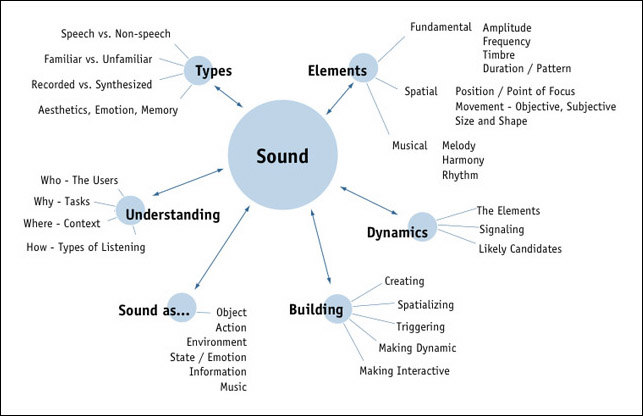
\includegraphics[width=.7\textwidth]{photo8_sound}
	\caption{The Complex Nature of Auditory Processing \cite{sound}}
	\label{fig:soundPerception}
\end{figure}

\par The challenge for auditory implementation in virtual environments stems from the complexity of auditory perception, illustrated in Figure \ref{fig:soundPerception}. Different types of sounds attract different types of attention. Ambient sounds give clues about the size and nature of an environment. The desired mood of an virtual environment is constructed through different ambient sounds. Individual objects can have sounds associated with them to give an understanding of each object and to demonstrate different possible actions that can accomplished with each object. Auditory processing is absolutely crucial but often overlooked in virtual settings due to the complexity of implementation. 

% speak about acoustic rendering? page 16 - haptics


\section{Design Guidelines} \label{Guidelines}




\section{Conclusion} \label{Guidelines}












%!TEX root = ../username.tex
\chapter{Interaction Systems}\label{interaction systems}


\section{Introduction to Unity}\label{Unity}
 
 Unity is a professional game engine that is used to create video games and virtual environments for a variety of platforms. Unity has two distinct advantages over other game development environments. The first is Unity's extremely user friendly visual workflow. Other game development tools are often overly complicated and require the user to set up their own integrated development environment, or IDE. Unity's visual editor is both sophisticated and extremely productive, allowing high quality games to be produced with relative ease and efficiency. The second advantage is Unity's wide array of cross-platform support. There are very few game engines that offer as many deployment targets, ranging from the PC, web and mobile to consoles. Unity also makes deploying to these platforms extremely simple. Compared to other game engines such as Unreal, CryEngine, or Game Maker, Unity stands in a fantastic middle ground in terms of the difficulty to learn and desired capabilities in engines. These comparisons and characteristics are brief examples of what makes Unity the engine of choice for many developers.
 
 \subsection{Unity's User Interface}
 
 Unity's user interface is split up into different tabs and sections as seen in Figure Blank
 
 %\ref{fig:UnityUI}. 
 
 The Project tab is used to view and access all the files in your project and the Console tab is available to view the output from your code. The Scene tab allows you to view the objects placed into the 3D scene and the Game tab lets you view the 3D scene as though the game is being played. The Hierarchy tab shows a list of all the objects in the scene and how they are nested in relation to each other. The Inspector tab displays information about the object selected and lets you change different components. The Toolbar provides scene navigation, including Move, Orbit, and Zoom functions. Unity's interface allows the user to easily create a 3D scene, however scripting is what brings a project to life. 
 
 %image insert
 
 \subsubsection{Scripting}
 
 \par Writing code in Unity is what controls your objects in the visual editor and makes the game interactive.  The game objects in Unity are built as a collection of components. This collection of components often include scripts, which refer to code files. Another nice aspect of Unity is code is not compiled and run as a separate executable, but instead executed within the Unity engine itself. Being able to test your game in a separate window without the inconvenience of having to create builds is very substantial. Unity supports both Javascript and C-sharp programming languages, although C-sharp is often preferred because it is strongly typed. When it comes time for writing scripts, picking an ideal IDE or text editor is important. Unity comes bundled with MonoDevelope, which is the IDE of choice because it is open source and offers cross-platform support for C-sharp. 

\subsection{Creating VR Through Unity}\label{creating VR through Unity}

\begin{figure}[h]
	\centering
	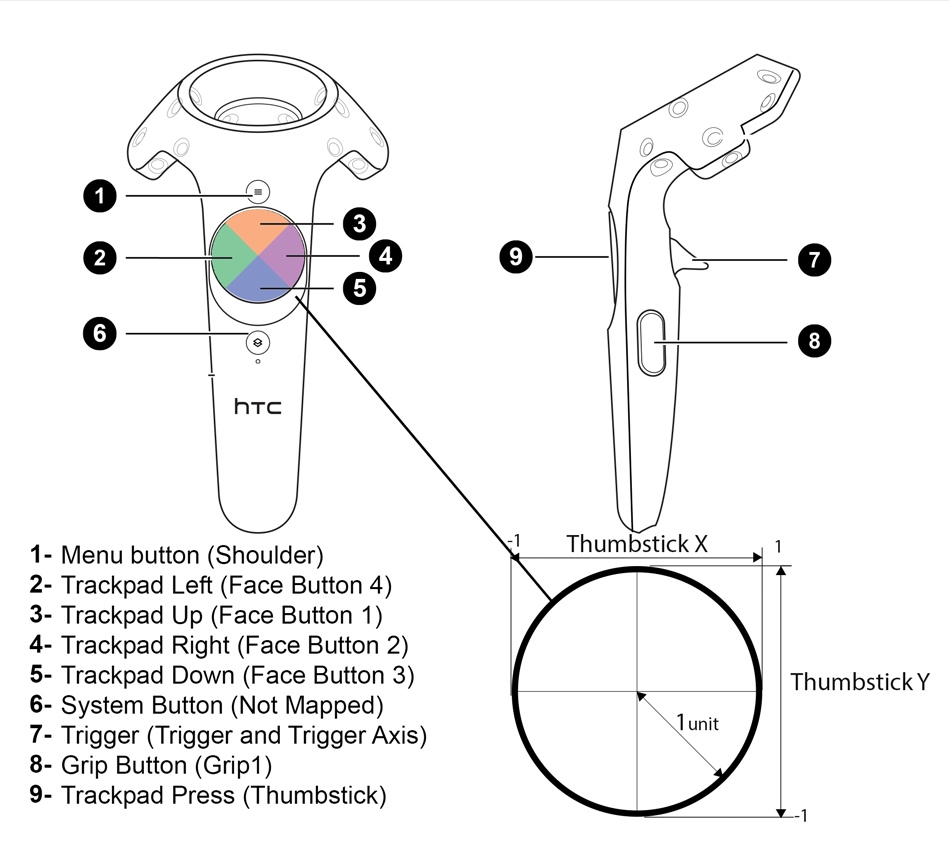
\includegraphics[width=.5\textwidth]{ViveControllers}
	\caption{Vive Controller Inputs \cite{ViveControllers}}
	\label{fig:ViveControllers}
\end{figure}

A distinct difference between virtual reality and an average game is the fact that when immersed in a virtual environment, quality is not just how good something looks, but how good something feels. Building an environment in Unity is one thing, but turning it into virtual reality involves a few extra steps. With a virtual reality application, different hardware is required, often with different types of input. With the HTC Vive, an effective user interface and realistic interaction systems must be implemented using the motion tracking capabilities and various input buttons on the Vive's controllers. Figure \ref{fig:ViveControllers} displays all the inputs that can be utilized by the controllers. 


\par A graphical user interface (GUI) is also essential for presenting information. A GUI refers to two-dimensional on screen graphics that overlay the main gameplay and present messages, gauges, or input controls such as menus buttons or sliders \cite{linowes}. In typical non VR games, a user interface is rendered in screen space, which statically rests somewhere on the screen as an overlay, such as a screen edge. In virtual reality, there are no screen edges, and the GUI must be rendered in what is called the World Space. Figure \ref{fig:GUI} shows a common approach taken by Oculus to display a main game menu. Although somewhat intrusive to the central scene, this style and placement for a GUI is easy to access a great alternative static main menu screen.

\begin{figure}[h]
	\centering
	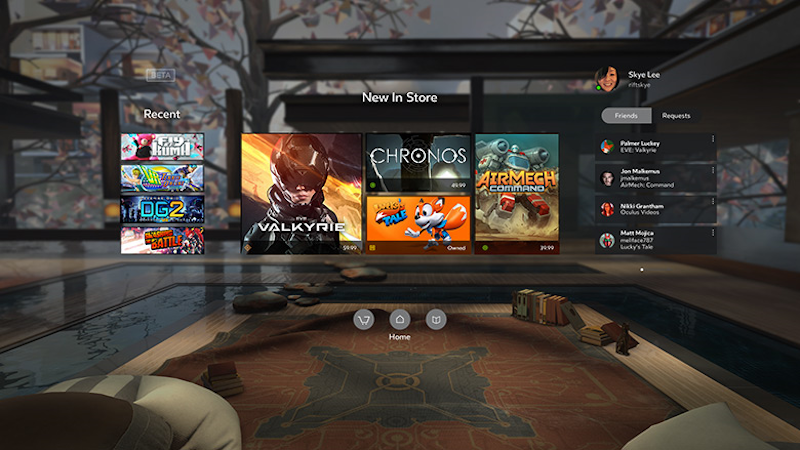
\includegraphics[width=.7\textwidth]{GUI}
	\caption{VR Game Menu - World Space \cite{GUI}}
	\label{fig:GUI}
\end{figure}




\subsection{VR Motion Sickness}

Despite the wonders of VR immersion, it is also known to cause feelings similar to motion sickness such as disorientation and nausea. VR motion sickness is a fairly substantial concern and is studied by many researchers, physiologists and technologists to find the underlying causes. We do know that lag caused by screen updates and synchronization problems when moving your head are a major contributing issue.
Given the potential impact rendering permanence, frames per second and latency have on a virtual reality application, optimizing implantation and content must be at the front of any developers mind \cite{gobbetti}. 
%Spatio-temporal realism, the ability to meet synchronization, lag, and accuracy constraints within low tolerates, has therefore become a required feature for virtual reality systems . 
Although these are the major issues corresponding to virtual reality motion sickness, there are a few others we should consider \cite{linowes}:

\begin{enumerate}
	\item Don't move too fast.
	\item Look forwards when moving through a scene.
	\item Avoid turning head too quickly.
	\item Use a third-person camera in certain settings.
	\item Provide visual cues to keep user grounded.
	\item Provide an option to recenter the view.
	\item Cut scenes break and transitions.
	\item Optimize rendering performance wherever possible.
\end{enumerate}

\section{Steam VR Plug-in}\label{steamVR}


\section{Naive System}\label{old}


\subsection{Allowances}\label{old _ allowances}


\subsection{Shortcomings}\label{old _ shortcomings}


\subsection{Improvements}\label{old _ improvements}


\section{Newtonian System}\label{new}


\subsection{Theory}\label{new _ theory}


\subsection{Allowances}\label{new _ allowances}


\subsection{Improvements}\label{new _ improvements}



%!TEX root = ../username.tex
\chapter{Implementation Theory}\label{Implementation Theory}

\section{Implementing New System}\label{implementing new system}


\subsection{Haptic API's}\label{API}

\subsection{NewtonVR Functions}\label{API}

\subsection{Deciding Which Objects Should be Interactable}\label{API}



\section{The Improvements}\label{Improvements with new system implemented}

\subsection{Low-Polly Worlds verse High Polly Worlds}\label{low polly vs. high polly}

\subsection{Better Immersion }\label{better immersion with new system implemented}

\section{Applications}\label{new system applications}
%!TEX root = ../username.tex
\chapter{Final Application Results}\label{results}

\section{Asset Pack Model}\label{Asset Pack}

\section{Applied Theory and Software}\label{applied theory and software}
%%!TEX root = ../username.tex
\chapter{Implementation Theory}\label{Implementation Theory}

\section{Implementing New System}\label{implementing new system}


\subsection{Haptic API's}\label{API}

\subsection{NewtonVR Functions}\label{API}

\subsection{Deciding Which Objects Should be Interactable}\label{API}



\section{The Improvements}\label{Improvements with new system implemented}

\subsection{Low-Polly Worlds verse High Polly Worlds}\label{low polly vs. high polly}

\subsection{Better Immersion }\label{better immersion with new system implemented}

\section{Applications}\label{new system applications}
%\input{chapters/chapter6}
%\input{chapters/chapter7}
%\input{conclusion}

%%%%%%%%%%%%%%%%%%%%%%%%%%%%%%%%%%%%%%%%%%%%%%%%%%%%%%%%%%%%%%%%%%%%%%%%%%%%%%%%%%%%%%%%%%%%%%
% This section starts the back matter. The back matter includes appendices, indicies, and the %bibliography
%%%%%%%%%%%%%%%%%%%%%%%%%%%%%%%%%%%%%%%%%%%%%%%%%%%%%%%%%%%%%%%%%%%%%%%%%%%%%%%%%%%%%%%%%%%%%%

\backmatter

%%!TEX root = ../username.tex
%%%%%%%%%%%%%%%%%%%%%%%%%%%%%%%%%%%%%%%%%%%%%%%%%%%%%%%%%%%%%%%%
% Contents: Math typesetting with LaTeX
% $Id: math.tex,v 1.3 2005/05/21 02:03:43 jonb Exp $
%%%%%%%%%%%%%%%%%%%%%%%%%%%%%%%%%%%%%%%%%%%%%%%%%%%%%%%%%%%%%%%%%

\chapter{Typesetting Mathematical Formulae}\label{math}
\begin{intro}
  This appendix is taken from \citet{ophs03} under the GNU open source documentation license. This appendix addresses the main strength
  of \TeX{}: mathematical typesetting. But be warned, this appendix
  only scratches the surface. While the things explained here are
  sufficient for many people, don't despair if you can't find a
  solution to your mathematical typesetting needs here. It is highly likely
  that your problem is addressed in \AmS-\LaTeX{}%
  \footnote{\texttt{CTAN:/tex-archive/macros/latex/packages/amslatex}}
  or some other package.
\end{intro}
  
\section{General}

\LaTeX{} has a special mode for typesetting mathematics\index{mathematics}.
Mathematical text within a paragraph is entered between \verb|\(|\index{\(@\verb+\(+}
and \verb|\)|\index{\)@\verb+\)+}, %$
between \texttt{\$} and \texttt{\$} or between
\verb|\begin{|{math}\verb|}| and \verb|\end{math}|.\index{formulae}

\begin{singlespace}
\begin{example}
Add $a$ squared and $b$ squared 
to get $c$ squared. Or, using 
a more mathematical approach:
$c^{2}=a^{2}+b^{2}$
\end{example}
\end{singlespace}

\begin{singlespace}
\begin{example}
\TeX{} is pronounced as 
$\tau\epsilon$.\\[6pt]
100~m$^{3}$ of water\\[6pt]
This comes from my $\heartsuit$
\end{example}
\end{singlespace}

It is preferable to \emph{display} larger mathematical equations or formulae,
rather than to typeset them on separate lines. This means you enclose them
in \verb|\[| \index{\[@\verb+\[+} and \verb|\]| \index{\]@\verb+\]+} or between
\verb|\begin{|displaymath\index{displaymath}\verb|}| and
  \verb|\end{displaymath}|.  This produces formulae which are not
numbered. If you want \LaTeX{} to number them, you can use the
equation\index{equation} environment.


\begin{singlespace}
\begin{example}
Add $a$ squared and $b$ squared 
to get $c$ squared. Or, using 
a more mathematical approach:
\begin{displaymath}
c^{2}=a^{2}+b^{2}
\end{displaymath}
And just one more line.
\end{example}
\end{singlespace}

You can reference an equation with \ic{label} and \ic{ref}

\begin{singlespace}
\begin{example}
\begin{equation} \label{eq:eps}
\epsilon > 0
\end{equation}
From (\ref{eq:eps}), we gather 
\ldots
\end{example}
\end{singlespace}

Note that expressions will be typeset in a different style if displayed:

\begin{singlespace}
\begin{example}
$\lim_{n \to \infty} 
\sum_{k=1}^n \frac{1}{k^2} 
= \frac{\pi^2}{6}$
\end{example}
\end{singlespace}
\begin{singlespace}
\begin{example}
\begin{displaymath}
\lim_{n \to \infty} 
\sum_{k=1}^n \frac{1}{k^2} 
= \frac{\pi^2}{6}
\end{displaymath}
\end{example}
\end{singlespace}

There are differences between \emph{math mode} and \emph{text mode}. For
example in \emph{math mode}: 

\begin{enumerate}

\item Most spaces and linebreaks do not have any significance, as all spaces
either are derived logically from the mathematical expressions or
have to be specified using special commands such as \verb|\,| \index{''\,@\verb+\,+}, \ic{quad}, or \ic{qquad}.
 
\item Empty lines are not allowed. Only one paragraph per formula.

\item Each letter is considered to be the name of a variable and will be
typeset as such. If you want to typeset normal text within a formula
(normal upright font and normal spacing) then you have to enter the
text using the \verb|\textrm{...}| commands.
\end{enumerate}


\begin{singlespace}
\begin{example}
\begin{equation}
\forall x \in \mathbf{R}:
\qquad x^{2} \geq 0
\end{equation}
\end{example}
\end{singlespace}

\begin{singlespace}
\begin{example}
\begin{equation}
x^{2} \geq 0\qquad
\textrm{for all }x\in\mathbf{R}
\end{equation}
\end{example}
\end{singlespace}

Mathematicians can be very fussy about which symbols are used:
it would be conventional here to use `blackboard bold\index{blackboard bold}',
bold symbols\index{bold symbols} which is obtained using \ic{mathbb} from the
package \ip{amsfonts} or \ip{amssymb}.

\ifx\mathbb\undefined\else
The last example becomes
\begin{singlespace}
\begin{example}
\begin{displaymath}
x^{2} \geq 0\qquad
\textrm{for all }x\in\mathbb{R}
\end{displaymath}
\end{example}
\end{singlespace}
\fi

\section{Grouping in Math Mode}

Most math mode commands act only on the next character. So if you
want a command to affect several characters, you have to group them
together using curly braces: \verb|{...}|.

\begin{singlespace}
\begin{example}
\begin{equation}
a^x+y \neq a^{x+y}
\end{equation}
\end{example}
\end{singlespace}
 
\section{Building Blocks of a Mathematical Formula}

In this section, the most important commands used in mathematical
typesetting will be described. Take a look at \citet{kd03} for a detailed list of commands for typesetting
mathematical symbols.

\textbf{Lowercase Greek letters\index{Greek letters}} are entered as \verb|\alpha|,
 \verb|\beta|, \verb|\gamma|, \ldots, uppercase letters
are entered as \verb|\Gamma|, \verb|\Delta|, \ldots\footnote{There is no
  uppercase Alpha defined in \LaTeXe{} because it looks the same as a
  normal roman A. Once the new math coding is done, things will
  change.} 

\begin{singlespace}
\begin{example}
$\lambda,\xi,\pi,\mu,\Phi,\Omega$
\end{example}
\end{singlespace}
 
\textbf{Exponents and Subscripts} can be specified using\index{exponent}\index{subscript}
the \verb|^|\index{^@\verb+^+} and the \verb|_|\index{_@\verb+_+} character.

\begin{singlespace}
\begin{example}
$a_{1}$ \qquad $x^{2}$ \qquad
$e^{-\alpha t}$ \qquad
$a^{3}_{ij}$\\
$e^{x^2} \neq {e^x}^2$
\end{example}
\end{singlespace}

The \textbf{square root\index{square root}} is entered as \ic{sqrt}, the
$n^\mathrm{th}$ root is generated with \verb|\sqrt[|$n$\verb|]|. The size of
the root sign is determined automatically by \LaTeX. If just the sign
is needed, use \ic{surd}.

\begin{singlespace}
\begin{example}
$\sqrt{x}$ \qquad 
$\sqrt{ x^{2}+\sqrt{y} }$ 
\qquad $\sqrt[3]{2}$\\[3pt]
$\surd[x^2 + y^2]$
\end{example}
\end{singlespace}

The commands \ic{overline} and \ic{underline} create
\textbf{horizontal lines} directly over or under an expression.
\index{horizontal!line}

\begin{singlespace}
\begin{example}
$\overline{m+n}$
\end{example}
\end{singlespace}

The commands \ic{overbrace} and \ic{underbrace} create
long \textbf{horizontal braces} over or under an expression.
\index{horizontal!brace}

\begin{singlespace}
\begin{example}
$\underbrace{ a+b+\cdots+z }_{26}$
\end{example}
\end{singlespace}

\index{mathematical!accents} To add mathematical accents such as small
arrows or {tilde} signs to variables, you can use the commands
given in \citet{kd03}.  Wide hats and
tildes covering several characters are generated with \ic{widetilde}
and \ic{widehat}.  The \verb|'|\index{'@\verb+'+} symbol gives a
prime\index{prime}.
% a dash is --

\begin{singlespace}
\begin{example}
\begin{displaymath}
y=x^{2}\qquad y'=2x\qquad y''=2
\end{displaymath}
\end{example}
\end{singlespace}

\textbf{Vectors}\index{vectors} often are specified by adding a small
arrow symbol\index{arrow symbols} on top of a variable. This is done with the
\ic{vec} command. The two commands \ic{overrightarrow} and
\ic{overleftarrow} are useful to denote the vector from $A$ to $B$.

\begin{singlespace}
\begin{example}
\begin{displaymath}
\vec a\quad\overrightarrow{AB}
\end{displaymath}
\end{example}
\end{singlespace}

Names of log-like functions are often typeset in an upright
font and not in italic like variables. Therefore \LaTeX{} supplies the
following commands to typeset the most important function names:
\index{mathematical!functions}

\begin{singlespace}
\begin{verbatim}
\arccos   \cos    \csc   \exp   \ker     \limsup  \min   \sinh
\arcsin   \cosh   \deg   \gcd   \lg      \ln      \Pr    \sup
\arctan   \cot    \det   \hom   \lim     \log     \sec   \tan
\arg      \coth   \dim   \inf   \liminf  \max     \sin   \tanh
\end{verbatim}
\end{singlespace}

\begin{singlespace}
\begin{example}
\[\lim_{x \rightarrow 0}
\frac{\sin x}{x}=1\]
\end{example}
\end{singlespace}

For the modulo function\index{modulo function}, there are two commands: \ic{bmod} for the
binary operator ``$a \bmod b$'' and \ic{pmod}
for expressions
such as ``$x\equiv a \pmod{b}$.''

A built-up \textbf{fraction\index{fraction}} is typeset with the
\ic{frac}\verb|{...}{...}| command.
Often the slashed form $1/2$ is preferable, because it looks better
for small amounts of `fraction material.'

\begin{singlespace}
\begin{example}
$1\frac{1}{2}$~hours
\begin{displaymath}
\frac{ x^{2} }{ k+1 }\qquad
x^{ \frac{2}{k+1} }\qquad
x^{ 1/2 }
\end{displaymath}
\end{example}
\end{singlespace}

To typeset binomial coefficients or similar structures, you can use
either the command \linebreak \ic{binom}\{\emph{num}\}\{\emph{denom}\} or \ic{genfrac}\{\emph{ldelim}\}\{\emph{rdelim}\}\{\emph{thickness}\}\{\emph{style}\}\{\emph{num}\}\{\emph{denom}\}. The second command can be used to produce customized fraction like output and more information can be found in \citet{mgbcr04}.

\begin{singlespace}
\begin{example}
\begin{displaymath}
\binom{n}{k}\qquad 
\genfrac{}{}{0pt}{}{x}{y+2}
\end{displaymath}
\end{example}
\end{singlespace}
 
\medskip

The \textbf{integral operator\index{integral operator}} is generated with \ic{int}, the
\textbf{sum operator\index{sum operator}} with \ic{sum}. The upper and lower limits
are specified with~\verb|^|\index{^@\verb+^+} and~\verb|_|\index{_@\verb+_+} like subscripts and superscripts.

\begin{singlespace}
\begin{example}
\begin{displaymath}
\sum_{i=1}^{n} \qquad
\int_{0}^{\frac{\pi}{2}} \qquad
\end{displaymath}
\end{example}
\end{singlespace}

For \textbf{braces\index{braces}} and other delimiters\index{delimiters}, there exist all
types of symbols in \TeX{} (e.g.~$[\;\langle\;\|\;\updownarrow$).
Round and square braces can be entered with the corresponding keys,
curly braces with \verb|\{|, all other delimiters are generated with
special commands (e.g.~\verb|\updownarrow|). For a list of all
delimiters available, check \citet{kd03}.

\begin{singlespace}
\begin{example}
\begin{displaymath}
{a,b,c}\neq\{a,b,c\}
\end{displaymath}
\end{example}
\end{singlespace}

If you put the command \ic{left} in front of an opening delimiter or
\ic{right} in front of a closing delimiter, \TeX{} will automatically
determine the correct size of the delimiter. Note that you must close
every \ic{left} with a corresponding \ic{right}, and that the size is
determined correctly only if both are typeset on the same line. If you
don't want anything on the right, use the invisible `\verb|\right .|\index{commands!right@\verb+right .+}'!

\begin{singlespace}
\begin{example}
\begin{displaymath}
1 + \left( \frac{1}{ 1-x^{2} }
    \right) ^3
\end{displaymath}
\end{example}
\end{singlespace}

In some cases it is necessary to specify the correct size of a
mathematical delimiter\index{mathematical!delimiter} by hand,
which can be done using the commands \ic{big}, \ic{Big}, \ic{bigg} and
\ic{Bigg} as prefixes to most delimiter commands.\footnote{These
  commands do not work as expected if a size changing command has been
  used, or the \texttt{11pt} or \texttt{12pt} option has been
  specified.  Use the exscale\index{exscale} or amsmath\index{amsmath} packages to
  correct this behaviour.}

\begin{singlespace}
\begin{example}
$\Big( (x+1) (x-1) \Big) ^{2}$\\
$\big(\Big(\bigg(\Bigg($\quad
$\big\}\Big\}\bigg\}\Bigg\}$\quad
$\big\|\Big\|\bigg\|\Bigg\|$
\end{example}
\end{singlespace}

To enter \textbf{three dots\index{three dots}} into a formula, you can use several
commands. \ic{ldots} typesets the dots on the baseline, \ic{cdots}
sets them centered. Besides that, there are the commands \ic{vdots} for
vertical and \ic{ddots} for diagonal dots\index{diagonal dots}.\index{vertical
  dots}\index{horizontal!dots} You can find another example in section~\ref{sec:vert}.

\begin{singlespace}
\begin{example}
\begin{displaymath}
x_{1},\ldots,x_{n} \qquad
x_{1}+\cdots+x_{n}
\end{displaymath}
\end{example}
\end{singlespace}
 
\section{Math Spacing}

\index{math spacing} If the spaces within formulae chosen by \TeX{}
are not satisfactory, they can be adjusted by inserting special
spacing commands. There are some commands for small spaces: \verb|\,| \index{\,@\verb+\,+} for
$\frac{3}{18}\:\textrm{quad}$ (\demowidth{0.166em}), \verb|\:| \index{\:@\verb+\:+} for $\frac{4}{18}\:
\textrm{quad}$ (\demowidth{0.222em}) and \verb|\;| \index{\;@\verb+\;+} for $\frac{5}{18}\:
\textrm{quad}$ (\demowidth{0.277em}).  The escaped space character
\verb*.\ . generates a medium sized space and \ic{quad}
(\demowidth{1em}) and \ic{qquad} (\demowidth{2em}) produce large
spaces. The size of a quad corresponds to the width of the
character `M' of the current font.  The \verb|\!|\index{"\"!@\texttt{\bs"!}} command produces a
negative space of $-\frac{3}{18}\:\textrm{quad}$ (\demowidth{0.166em}).

\begin{singlespace}
\begin{example}
\newcommand{\rd}{\mathrm{d}}
\begin{displaymath}
\int\!\!\!\int_{D} g(x,y)
  \, \rd x\, \rd y 
\end{displaymath}
instead of 
\begin{displaymath}
\int\int_{D} g(x,y)\rd x \rd y
\end{displaymath}
\end{example}
\end{singlespace}
Note that `d' in the differential is conventionally set in roman.

\AmS-\LaTeX{} provides another way for fine tuning
the spacing between multiple integral signs,
namely the \ic{iint}, \ic{iiint}, \ic{iiiint}, and \ic{idotsint} commands.
With the \ip{amsmath} package loaded, the above example can be
typeset this way:

\begin{singlespace}
\begin{example}
\newcommand{\rd}{\mathrm{d}}
\begin{displaymath}
\iint_{D} \, \rd x \, \rd y
\end{displaymath}
\end{example}
\end{singlespace}

See the electronic document testmath.tex (distributed with
\AmS-\LaTeX) or Chapter 8 of ``The LaTeX Companion''\footnote{
available at \texttt{CTAN:/tex-archive/info/ch8.*}.} for further details.

\section{Vertically Aligned Material}
\label{sec:vert}

To typeset \textbf{arrays}, use the \texttt{array}\index{array} environment. It works
somewhat similar to the \texttt{tabular} environment. The \verb|\\| command is
used to break the lines.

\begin{singlespace}
\begin{example}
\begin{displaymath}
\mathbf{X} =
\left( \begin{array}{ccc}
x_{11} & x_{12} & \ldots \\
x_{21} & x_{22} & \ldots \\
\vdots & \vdots & \ddots
\end{array} \right)
\end{displaymath}
\end{example}
\end{singlespace}

The \texttt{array}\index{array} environment can also be used to typeset expressions which have one
big delimiter by using a ``\verb|.|'' as an invisible right\index{commands!right@\verb+right .+} 
delimiter:

\begin{singlespace}
\begin{example}
\begin{displaymath}
y = \left\{ \begin{array}{ll}
 a & \textrm{if $d>c$}\\
 b+x & \textrm{in the morning}\\
 l & \textrm{all day long}
  \end{array} \right.
\end{displaymath}
\end{example}
\end{singlespace}


For formulae running over several lines or for equation systems\index{equation systems},
you can use the environments \texttt{eqnarray}\index{eqnarray}, and \verb|eqnarray*|
instead of \texttt{equation}. In \texttt{eqnarray} each line gets an
equation number. The \verb|eqnarray*| does not number anything.

The \texttt{eqnarray} and the \verb|eqnarray*| environments work like
a 3-column table of the form \verb|{rcl}|, where the middle column can
be used for the equal sign or the not-equal sign. Or any other sign
you see fit. The \verb|\\| command breaks the lines.

\begin{singlespace}
\begin{example}
\begin{eqnarray}
f(x) & = & \cos x     \\
f'(x) & = & -\sin x   \\
\int_{0}^{x} f(y)dy &
 = & \sin x
\end{eqnarray}
\end{example}
\end{singlespace}

\noindent Notice that the space on either side of the 
the equal signs is rather large. It can be reduced by setting
\verb|\setlength\arraycolsep{2pt}|, as in the next example.

\index{long equations} \textbf{Long equations} will not be
automatically divided into neat bits.  The author has to specify
where to break them and how much to indent. The following two methods
are the most common ones used to achieve this.

\begin{singlespace}
\begin{example}
{\setlength\arraycolsep{2pt}
\begin{eqnarray}\notag
\sin x & = & x -\frac{x^{3}}{3!}
     +\frac{x^{5}}{5!}-{}
                   \\\notag
 & & {}-\frac{x^{7}}{7!}+{}\cdots
\end{eqnarray}}
\end{example}
\end{singlespace}
\pagebreak[1]

\begin{singlespace}
\begin{example}
\begin{eqnarray}\notag
\lefteqn{ \cos x = 1
     -\frac{x^{2}}{2!} +{} }
                   \\\notag
 & & {}+\frac{x^{4}}{4!}
     -\frac{x^{6}}{6!}+{}\cdots
\end{eqnarray}
\end{example}
\end{singlespace}

\enlargethispage{\baselineskip}

\noindent The \ic{notag} command causes \LaTeX{} to not generate a number for
this equation.

It can be difficult to get vertically aligned equations to look right
with these methods; the package amsmath\index{amsmath} provides a more
powerful set of alternatives.

\section{Math Font Size}

\index{math font size} In math mode, \TeX{} selects the font size
according to the context. Superscripts, for example, get typeset in a
smaller font. If you want to typeset part of an equation in roman,
don't use the \ic{textrm} command, because the font size switching
mechanism will not work, as \verb|\textrm| temporarily escapes to text
mode. Use \verb|\mathrm| instead to keep the size switching mechanism
active. But pay attention, \ic{mathrm} will only work well on short
items. Spaces are still not active and accented characters do not
work.\footnote{The \AmS-\LaTeX{} package makes the textrm command
  work with size changing.}

\begin{singlespace}
\begin{example}
\begin{equation}
2^{\textrm{nd}} \quad 
2^{\mathrm{nd}}
\end{equation}
\end{example}
\end{singlespace}

Nevertheless, sometimes you need to tell \LaTeX{} the correct font
size. In math mode, the font size is set with the four commands:
\begin{center}
{displaystyle}~($\displaystyle 123$),
{textstyle}~($\textstyle 123$), 
{scriptstyle}~($\scriptstyle 123$) and
{scriptscriptstyle}~($\scriptscriptstyle 123$).
\end{center}

Changing styles also affects the way limits are displayed.

\begin{singlespace}
\begin{example}
\begin{displaymath}
\mathop{\mathrm{corr}}(X,Y)= 
 \frac{\displaystyle 
   \sum_{i=1}^n(x_i-\overline x)
   (y_i-\overline y)} 
  {\displaystyle\biggl[
 \sum_{i=1}^n(x_i-\overline x)^2
\sum_{i=1}^n(y_i-\overline y)^2
\biggr]^{1/2}}
\end{displaymath}    
\end{example}
\end{singlespace}
% This is not a math accent, and no maths book would be set this way.
% mathop gets the spacing right.

\noindent This is one of those examples in which we need larger
brackets than the standard \verb|\left[  \right]| provides.


\section{Theorems, Laws, \ldots}

When writing mathematical documents, you probably need a way to
typeset ``Lemmas'', ``Definitions'', ``Axioms'' and similar
structures. \LaTeX{} supports this with the command
\begin{command}
{newtheorem}\verb|{|\emph{name}\verb|}[|\emph{counter}\verb|]{|%
         \emph{text}\verb|}[|\emph{section}\verb|]|
\end{command}
The \emph{name} argument, is a short keyword used to identify the
``theorem''. With the \emph{text} argument, you define the actual name
of the ``theorem'' which will be printed in the final document.

The arguments in square brackets are optional. They are both used to
specify the numbering used on the ``theorem''. With the \emph{counter}
argument you can specify the \emph{name} of a previously declared
``theorem''. The new ``theorem'' will then be numbered in the same
sequence.  The \emph{section} argument allows you to specify the
sectional unit within which you want your ``theorem'' to be numbered.

After executing the {newtheorem} command in the preamble of your
document, you can use the following command within the document.

\begin{code}
\verb|\begin{|\emph{name}\verb|}[|\emph{text}\verb|]|\\
This is my interesting theorem\\
\verb|\end{|\emph{name}\verb|}|     
\end{code}

This should be enough theory. The following examples will hopefully
remove the final remains of doubt and make it clear that the
\verb|\newtheorem| environment is way too complex to understand.

\begin{singlespace}
\begin{example}
% definitions for the document
% preamble
\newtheorem{law}{Law}
\newtheorem{jury}[law]{Jury}
%in the document
\begin{law} \label{law:box}
Don't hide in the witness box
\end{law}
\begin{jury}[The Twelve]
It could be you! So beware and
see law~\ref{law:box}\end{jury}
\begin{law}No, No, No\end{law}
\end{example}
\end{singlespace}

The ``Jury'' theorem uses the same counter as the ``Law''
theorem. Therefore it gets a number which is in sequence with
the other ``Laws''. The argument in square brackets is used to specify 
a title or something similar for the theorem.

\begin{singlespace}
\begin{example}
\flushleft
\newtheorem{mur}{Murphy}[section]
\begin{mur}
If there are two or more 
ways to do something, and 
one of those ways can result 
in a catastrophe, then 
someone will do it.\end{mur}
\end{example}
\end{singlespace}

The ``Murphy'' theorem gets a number which is linked to the number of
the current section. You could also use another unit, for example chapter or
subsection.

\section{Bold symbols}
\index{bold symbols}

It is quite difficult to get bold symbols in \LaTeX{}; this is 
probably intentional as amateur typesetters tend to overuse them.
The font change command \verb|\mathbf| gives bold letters, but these are
roman (upright) whereas mathematical symbols are normally italic.
There is a \ic{boldmath} command, but \emph{this can only be
used outside mathematics mode}. It works for symbols too.

\begin{singlespace}
\begin{example}
\begin{displaymath}
\mu, M \qquad \mathbf{M} \qquad
\mbox{\boldmath $\mu, M$}
\end{displaymath}
\end{example}
\end{singlespace}

\noindent
Notice that the comma is bold too, which may not be what is required.

The package \ip{amsbsy} (included by \ip{amsmath}) makes this much
easier as it includes a \ic{boldsymbol} command.

\ifx\boldsymbol\undefined\else
\begin{singlespace}
\begin{example}
\begin{displaymath}
\mu, M \qquad
\boldsymbol{\mu}, \boldsymbol{M}
\end{displaymath}
\end{example}
\end{singlespace}
\fi

\section{List of Mathematical Symbols}  \label{symbols}
 
In the following tables, you find all the symbols normally accessible
from \emph{math mode}.  

%
% Conditional Text in case the AMS Fonts are installed
%
\ifx\noAMS\relax To use the symbols listed in
Tables~\ref{AMSD}--\ref{AMSNBR},\footnote{These tables were derived
  from \texttt{symbols.tex} by David~Carlisle and subsequently changed
extensively as suggested by Josef~Tkadlec.} the package
\ip{amssymb} must be loaded in the preamble of the document and the
AMS math fonts must be installed, on the system. If the AMS package and
fonts are not installed, on your system, have a look at\\ 
\texttt{CTAN:/tex-archive/macros/latex/required/amslatex}\fi
 
\begin{table}[!ht]
\caption{Math Mode Accents.}  \label{mathacc}
\begin{symbols}{*4{cl}}
\W{\hat}{a}     & \W{\check}{a} & \W{\tilde}{a} & \W{\acute}{a} \\
\W{\grave}{a} & \W{\dot}{a} & \W{\ddot}{a}    & \W{\breve}{a} \\
\W{\bar}{a} &\W{\vec}{a} &\W{\widehat}{A}&\W{\widetilde}{A}\\  
\end{symbols}
\end{table}
 
\begin{table}[!ht]
\caption{Lowercase Greek Letters.}
\begin{symbols}{*4{cl}}
 \X{\alpha}     & \X{\theta}     & \X{o}          & \X{\upsilon}  \\
 \X{\beta}      & \X{\vartheta}  & \X{\pi}        & \X{\phi}      \\
 \X{\gamma}     & \X{\iota}      & \X{\varpi}     & \X{\varphi}   \\
 \X{\delta}     & \X{\kappa}     & \X{\rho}       & \X{\chi}      \\
 \X{\epsilon}   & \X{\lambda}    & \X{\varrho}    & \X{\psi}      \\
 \X{\varepsilon}& \X{\mu}        & \X{\sigma}     & \X{\omega}    \\
 \X{\zeta}      & \X{\nu}        & \X{\varsigma}  & &             \\
 \X{\eta}       & \X{\xi}        & \X{\tau} 
\end{symbols}
\end{table}

\begin{table}[!ht]
\caption{Uppercase Greek Letters.}
\begin{symbols}{*4{cl}}
 \X{\Gamma}     & \X{\Lambda}    & \X{\Sigma}     & \X{\Psi}      \\
 \X{\Delta}     & \X{\Xi}        & \X{\Upsilon}   & \X{\Omega}    \\
 \X{\Theta}     & \X{\Pi}        & \X{\Phi} 
\end{symbols}
\end{table}
\clearpage 

\begin{table}[!tbp]
\caption{Binary Relations.}
\bigskip
You can produce corresponding negations by adding a \verb|\not| command
as prefix to the following symbols.
\begin{symbols}{*3{cl}}
 \X{<}           & \X{>}           & \X{=}          \\
 \X{\leq}or \verb|\le|   & \X{\geq}or \verb|\ge|   & \X{\equiv}     \\
 \X{\ll}         & \X{\gg}         & \X{\doteq}     \\
 \X{\prec}       & \X{\succ}       & \X{\sim}       \\
 \X{\preceq}     & \X{\succeq}     & \X{\simeq}     \\
 \X{\subset}     & \X{\supset}     & \X{\approx}    \\
 \X{\subseteq}   & \X{\supseteq}   & \X{\cong}      \\
 \X{\sqsubset}$^a$ & \X{\sqsupset}$^a$ & \X{\Join}$^a$    \\
 \X{\sqsubseteq} & \X{\sqsupseteq} & \X{\bowtie}    \\
 \X{\in}         & \X{\ni}, \verb|\owns|  & \X{\propto}    \\
 \X{\vdash}      & \X{\dashv}      & \X{\models}    \\
 \X{\mid}        & \X{\parallel}   & \X{\perp}      \\
 \X{\smile}      & \X{\frown}      & \X{\asymp}     \\
 \X{:}           & \X{\notin}      & \X{\neq}or \verb|\ne|
\end{symbols}
\centerline{\footnotesize $^a$Use the \texttt{latexsym} package to access this symbol}
\end{table}

\begin{table}[!tbp]
\caption{Binary Operators.}
\begin{symbols}{*3{cl}}
 \X{+}              & \X{-}              & &                 \\
 \X{\pm}            & \X{\mp}            & \X{\triangleleft} \\
 \X{\cdot}          & \X{\div}           & \X{\triangleright}\\
 \X{\times}         & \X{\setminus}      & \X{\star}         \\
 \X{\cup}           & \X{\cap}           & \X{\ast}          \\
 \X{\sqcup}         & \X{\sqcap}         & \X{\circ}         \\
 \X{\vee}, \verb|\lor|     & \X{\wedge}, \verb|\land|  & \X{\bullet}       \\
 \X{\oplus}         & \X{\ominus}        & \X{\diamond}      \\
 \X{\odot}          & \X{\oslash}        & \X{\uplus}        \\
 \X{\otimes}        & \X{\bigcirc}       & \X{\amalg}        \\
 \X{\bigtriangleup} &\X{\bigtriangledown}& \X{\dagger}       \\
 \X{\lhd}$^a$         & \X{\rhd}$^a$         & \X{\ddagger}      \\
 \X{\unlhd}$^a$       & \X{\unrhd}$^a$       & \X{\wr}
\end{symbols}
 
\end{table}

\begin{table}[!tbp]
\caption{BIG Operators.}
\begin{symbols}{*4{cl}}
 \X{\sum}      & \X{\bigcup}   & \X{\bigvee}   & \X{\bigoplus}\\
 \X{\prod}     & \X{\bigcap}   & \X{\bigwedge} &\X{\bigotimes}\\
 \X{\coprod}   & \X{\bigsqcup} & &             & \X{\bigodot} \\
 \X{\int}      & \X{\oint}     & &             & \X{\biguplus}
\end{symbols}
 
\end{table}


\begin{table}[!tbp]
\caption{Arrows.}
\begin{symbols}{*3{cl}}
 \X{\leftarrow}or \verb|\gets|& \X{\longleftarrow}     & \X{\uparrow}          \\
 \X{\rightarrow}or \verb|\to|& \X{\longrightarrow}    & \X{\downarrow}        \\
 \X{\leftrightarrow}    & \X{\longleftrightarrow}& \X{\updownarrow}      \\
 \X{\Leftarrow}         & \X{\Longleftarrow}     & \X{\Uparrow}          \\
 \X{\Rightarrow}        & \X{\Longrightarrow}    & \X{\Downarrow}        \\
 \X{\Leftrightarrow}    & \X{\Longleftrightarrow}& \X{\Updownarrow}      \\
 \X{\mapsto}            & \X{\longmapsto}        & \X{\nearrow}          \\
 \X{\hookleftarrow}     & \X{\hookrightarrow}    & \X{\searrow}          \\
 \X{\leftharpoonup}     & \X{\rightharpoonup}    & \X{\swarrow}          \\
 \X{\leftharpoondown}   & \X{\rightharpoondown}  & \X{\nwarrow}          \\
 \X{\rightleftharpoons} & \X{\iff}(bigger spaces)& \X{\leadsto}$^a$

\end{symbols}
\centerline{\footnotesize $^a$Use the \texttt{latexsym} package to access this symbol}
\end{table}

\begin{table}[!tbp]
\caption{Delimiters.}\label{tab:delimiters}
\begin{symbols}{*4{cl}}
 \X{(}            & \X{)}            & \X{\uparrow} & \X{\Uparrow}    \\
 \X{[}or \verb|\lbrack|   & \X{]}or \verb|\rbrack|  & \X{\downarrow}   & \X{\Downarrow}  \\
 \X{\{}or \verb|\lbrace|  & \X{\}}or \verb|\rbrace|  & \X{\updownarrow} & \X{\Updownarrow}\\
 \X{\langle}      & \X{\rangle}  & \X{|}or \verb|\vert| &\X{\|}or \verb|\Vert|\\
 \X{\lfloor}      & \X{\rfloor}      & \X{\lceil}       & \X{\rceil}      \\
 \X{/}            & \X{\backslash}   & &. (dual. empty)
\end{symbols}
\end{table}

\begin{table}[!tbp]
\caption{Large Delimiters.}
\begin{symbols}{*4{cl}}
 \Y{\lgroup}      & \Y{\rgroup}      & \Y{\lmoustache}  & \Y{\rmoustache} \\
 \Y{\arrowvert}   & \Y{\Arrowvert}   & \Y{\bracevert} 
\end{symbols}
\end{table}


\begin{table}[!tbp]
\caption{Miscellaneous Symbols.}
\begin{symbols}{*4{cl}}
 \X{\dots}       & \X{\cdots}      & \X{\vdots}      & \X{\ddots}     \\
 \X{\hbar}       & \X{\imath}      & \X{\jmath}      & \X{\ell}       \\
 \X{\Re}         & \X{\Im}         & \X{\aleph}      & \X{\wp}        \\
 \X{\forall}     & \X{\exists}     & \X{\mho}$^a$      & \X{\partial}   \\
 \X{'}           & \X{\prime}      & \X{\emptyset}   & \X{\infty}     \\
 \X{\nabla}      & \X{\triangle}   & \X{\Box}$^a$     & \X{\Diamond}$^a$ \\
 \X{\bot}        & \X{\top}        & \X{\angle}      & \X{\surd}      \\
\X{\diamondsuit} & \X{\heartsuit}  & \X{\clubsuit}   & \X{\spadesuit} \\
 \X{\neg}or \verb|\lnot| & \X{\flat}       & \X{\natural}    & \X{\sharp}

\end{symbols}
\centerline{\footnotesize $^a$Use the \texttt{latexsym} package to access this symbol}
\end{table}

\begin{table}[!tbp]
\caption{Non-Mathematical Symbols.}
\bigskip
These symbols can also be used in text mode.
\begin{symbols}{*3{cl}}
\SC{\dag} & \SC{\S} & \SC{\copyright}  \\
\SC{\ddag} & \SC{\P} & \SC{\pounds}  \\
\end{symbols}
\end{table}

%
%
% If the AMS Stuff is not available, we drop out right here :-)
%
\noAMS

\begin{table}[!tbp]
\caption{AMS Delimiters.}\label{AMSD}
\bigskip
\begin{symbols}{*4{cl}}
\X{\ulcorner}&\X{\urcorner}&\X{\llcorner}&\X{\lrcorner}
\end{symbols}
\end{table}

\begin{table}[!tbp]
\caption{AMS Greek and Hebrew.}
\begin{symbols}{*5{cl}}
\X{\digamma}     &\X{\varkappa} & \X{\beth}& \X{\daleth}     &\X{\gimel}
\end{symbols}
\end{table}

\begin{table}[!tbp]
\caption{AMS Binary Relations.}
\begin{symbols}{*3{cl}}
 \X{\lessdot}           & \X{\gtrdot}            & \X{\doteqdot}or \verb|\Doteq| \\
 \X{\leqslant}          & \X{\geqslant}          & \X{\risingdotseq}     \\
 \X{\eqslantless}       & \X{\eqslantgtr}        & \X{\fallingdotseq}    \\
 \X{\leqq}              & \X{\geqq}              & \X{\eqcirc}           \\
 \X{\lll}or \verb|\llless|      & \X{\ggg}or \verb|\gggtr| & \X{\circeq}  \\
 \X{\lesssim}           & \X{\gtrsim}            & \X{\triangleq}        \\
 \X{\lessapprox}        & \X{\gtrapprox}         & \X{\bumpeq}           \\
 \X{\lessgtr}           & \X{\gtrless}           & \X{\Bumpeq}           \\
 \X{\lesseqgtr}         & \X{\gtreqless}         & \X{\thicksim}         \\
 \X{\lesseqqgtr}        & \X{\gtreqqless}        & \X{\thickapprox}      \\
 \X{\preccurlyeq}       & \X{\succcurlyeq}       & \X{\approxeq}
 \end{symbols}
 \end{table}
 
 \begin{table}[!tbp]
\caption{AMS Binary Relations Continued.}
\begin{symbols}{*3{cl}}
 \X{\curlyeqprec}       & \X{\curlyeqsucc}       & \X{\backsim}          \\
 \X{\precsim}           & \X{\succsim}           & \X{\backsimeq}        \\
 \X{\precapprox}        & \X{\succapprox}        & \X{\vDash}            \\
 \X{\subseteqq}         & \X{\supseteqq}         & \X{\Vdash}            \\
 \X{\Subset}            & \X{\Supset}            & \X{\Vvdash}           \\
 \X{\sqsubset}          & \X{\sqsupset}          & \X{\backepsilon}      \\
 \X{\therefore}         & \X{\because}           & \X{\varpropto}        \\
 \X{\shortmid}          & \X{\shortparallel}     & \X{\between}          \\
 \X{\smallsmile}        & \X{\smallfrown}        & \X{\pitchfork}        \\
 \X{\vartriangleleft}   & \X{\vartriangleright}  & \X{\blacktriangleleft}\\
 \X{\trianglelefteq}    & \X{\trianglerighteq}   &\X{\blacktriangleright}
\end{symbols}
\end{table}

\begin{table}[!tbp]
\caption{AMS Arrows.}
\begin{symbols}{*3{cl}}
 \X{\dashleftarrow}      & \X{\dashrightarrow}     & \X{\multimap}          \\
 \X{\leftleftarrows}     & \X{\rightrightarrows}   & \X{\upuparrows}        \\
 \X{\leftrightarrows}    & \X{\rightleftarrows}    & \X{\downdownarrows}    \\
 \X{\Lleftarrow}         & \X{\Rrightarrow}        & \X{\upharpoonleft}     \\
 \X{\twoheadleftarrow}   & \X{\twoheadrightarrow}  & \X{\upharpoonright}    \\
 \X{\leftarrowtail}      & \X{\rightarrowtail}     & \X{\downharpoonleft}   \\
 \X{\leftrightharpoons}  & \X{\rightleftharpoons}  & \X{\downharpoonright}  \\
 \X{\Lsh}                & \X{\Rsh}                & \X{\rightsquigarrow}   \\
 \X{\looparrowleft}      & \X{\looparrowright}     &\X{\leftrightsquigarrow}\\
 \X{\curvearrowleft}     & \X{\curvearrowright}    & &                      \\
 \X{\circlearrowleft}    & \X{\circlearrowright}   & &
\end{symbols}
\end{table}

\begin{table}[!tbp]
\caption{AMS Negated Binary Relations and Arrows.}\label{AMSNBR}
\begin{symbols}{*3{cl}}
 \X{\nless}           & \X{\ngtr}            & \X{\varsubsetneqq}  \\
 \X{\lneq}            & \X{\gneq}            & \X{\varsupsetneqq}  \\[-0.5ex]
 \X{\nleq}            & \X{\ngeq}            & \X{\nsubseteqq}     \\
 \X{\nleqslant}       & \X{\ngeqslant}       & \X{\nsupseteqq}     \\[-0.5ex]
 \X{\lneqq}           & \X{\gneqq}           & \X{\nmid}           \\
 \X{\lvertneqq}       & \X{\gvertneqq}       & \X{\nparallel}      \\[-0.5ex]
 \X{\nleqq}           & \X{\ngeqq}           & \X{\nshortmid}      \\
 \X{\lnsim}           & \X{\gnsim}           & \X{\nshortparallel} \\[-0.5ex]
 \X{\lnapprox}        & \X{\gnapprox}        & \X{\nsim}           \\
 \X{\nprec}           & \X{\nsucc}           & \X{\ncong}          \\[-0.5ex]
 \X{\npreceq}         & \X{\nsucceq}         & \X{\nvdash}         \\
 \X{\precneqq}        & \X{\succneqq}        & \X{\nvDash}         \\[-0.5ex]
 \X{\precnsim}        & \X{\succnsim}        & \X{\nVdash}         \\
 \X{\precnapprox}     & \X{\succnapprox}     & \X{\nVDash}         \\[-0.5ex]
 \X{\subsetneq}       & \X{\supsetneq}       & \X{\ntriangleleft}  \\
 \X{\varsubsetneq}    & \X{\varsupsetneq}    & \X{\ntriangleright} \\[-0.5ex]
 \X{\nsubseteq}       & \X{\nsupseteq}       & \X{\ntrianglelefteq}\\
 \X{\subsetneqq}      & \X{\supsetneqq}      &\X{\ntrianglerighteq}\\[-0.5ex]
 \X{\nleftarrow}      & \X{\nrightarrow}     & \X{\nleftrightarrow}\\
 \X{\nLeftarrow}      & \X{\nRightarrow}     & \X{\nLeftrightarrow}
\end{symbols}
\end{table}

\begin{table}[!tbp]
\caption{AMS Binary Operators.}
\begin{symbols}{*3{cl}}
 \X{\dotplus}        & \X{\centerdot}      & \X{\intercal}      \\
 \X{\ltimes}         & \X{\rtimes}         & \X{\divideontimes} \\
 \X{\Cup}or \verb|\doublecup|& \X{\Cap}or \verb|\doublecap|& \X{\smallsetminus} \\
 \X{\veebar}         & \X{\barwedge}       & \X{\doublebarwedge}\\
 \X{\boxplus}        & \X{\boxminus}       & \X{\circleddash}   \\
 \X{\boxtimes}       & \X{\boxdot}         & \X{\circledcirc}   \\
 \X{\leftthreetimes} & \X{\rightthreetimes}& \X{\circledast}    \\
 \X{\curlyvee}       & \X{\curlywedge}  
\end{symbols}
\end{table}

\begin{table}[!tbp]
\caption{AMS Miscellaneous.}
\begin{symbols}{*3{cl}}
 \X{\hbar}             & \X{\hslash}           & \X{\Bbbk}            \\
 \X{\square}           & \X{\blacksquare}      & \X{\circledS}        \\
 \X{\vartriangle}      & \X{\blacktriangle}    & \X{\complement}      \\
 \X{\triangledown}     &\X{\blacktriangledown} & \X{\Game}            \\
 \X{\lozenge}          & \X{\blacklozenge}     & \X{\bigstar}         \\
 \X{\angle}            & \X{\measuredangle}    & \X{\sphericalangle}  \\
 \X{\diagup}           & \X{\diagdown}         & \X{\backprime}       \\
 \X{\nexists}          & \X{\Finv}             & \X{\varnothing}      \\
 \X{\eth}              & \X{\mho}       
\end{symbols}
\end{table}



\begin{table}[!tbp]
\caption{Math Alphabets.}
\begin{symbols}{@{}*3l@{}}
Example& Command &Required package\\
\hline
\rule{0pt}{1.05em}$\mathrm{ABCdef}$
        & \verb|\mathrm{ABCdef}|
        &       \\
$\mathit{ABCdef}$
        & \verb|\mathit{ABCdef}|
        &       \\
$\mathnormal{ABCdef}$
        & \verb|\mathnormal{ABCdef}|
        &       \\
$\mathcal{ABC}$
        & \verb|\mathcal{ABC}|
        &       \\
\ifx\MathRSFS\undefined\else
$\MathRSFS{ABC}$
        &\verb|\mathcal{ABC}|
        &\pai{mathrsfs}\\
\fi
\ifx\EuScript\undefined\else
$\EuScript{ABC}$
        & \verb|\mathcal{ABC}|
        &\ip{eucal} with option: \index{mathcal}  \quad or\\
        & \verb|\mathscr{ABC}|  
        &\ip{eucal}  with option: mathscr\index{mathscr}\\
$\mathfrak{ABCdef}$
        & \verb|\mathfrak{ABCdef}|
        &\ip{eufrak}                \\
\fi
$\mathbb{ABC}$
        & \verb|\mathbb{ABC}|
        &\ip{amsfonts} or \ip{amssymb}        \\
\end{symbols}
\end{table}

%%% Local Variables: 
%%% mode: latex
%%% TeX-master: "lshort2e"
%%% End: 



%%!TEX root = ../username.tex
\chapter{Examples of Java Code}
Here are some examples of Java source using the \texttt{listings} package. I have entered the following before any code examples to format the code as shown.

\begin{singlespace}
\begin{verbatim}
\lstset{language=java}
\lstset{backgroundcolor=\color{white},rulecolor=\color{black}}
\lstset{linewidth=.95\textwidth,breaklines=true}
\lstset{commentstyle=\textit,stringstyle=\upshape,showspaces=false}
\lstset{frame = trbl, frameround=tttt}
\lstset{numbers=left,numberstyle=\tiny,basicstyle=\small}
\lstset{commentstyle=\normalfont\itshape,breakautoindent=true}
\lstset{abovecaptionskip=1.2\baselineskip,xleftmargin=30pt}
\lstset{framesep=6pt}
\end{verbatim}
\end{singlespace}

I have included the code by entering
\begin{singlespace}
\begin{verbatim}
\begin{singlespace}
\lstinputlisting[caption=Clock Code,label=clock]{source/Clock.java}
\end{singlespace}
\end{verbatim}
\end{singlespace}

\lstset{language=java}
\lstset{backgroundcolor=\color{white},rulecolor=\color{black}}
\lstset{linewidth=.95\textwidth,breaklines=true}
\lstset{commentstyle=\textit,stringstyle=\upshape,showspaces=false}
\lstset{frame = trbl, frameround=tttt}
\lstset{numbers=left,numberstyle=\tiny,basicstyle=\small}
\lstset{commentstyle=\normalfont\itshape,breakautoindent=true}
\lstset{abovecaptionskip=1.2\baselineskip,xleftmargin=30pt}
\lstset{framesep=6pt}

\begin{singlespace}
\lstinputlisting[caption=Clock Code, label=clock]{source/Clock.java}
\end{singlespace}
\newpage

\begin{singlespace}
\lstinputlisting[caption=Consumer, label=consumer]{source/Consumer.java}
\end{singlespace}

\begin{singlespace}
\lstinputlisting[caption=EvilEmpire Code, label=evil]{source/EvilEmpire.java}
\end{singlespace}

%%!TEX root = ../username.tex
\chapter{C++ Examples}
This appendix demonstrates the \texttt{listings} packages ability to format C++ code.

\lstset{language =[ANSI]C++}
\lstset{backgroundcolor=\color{white},rulecolor=\color{black}}
\lstset{linewidth=.95\textwidth,breaklines=true}
\lstset{commentstyle=\textit,stringstyle=\upshape,showspaces=false}
\lstset{frame = trbl, frameround=tttt}
\lstset{numbers=left,numberstyle=\tiny,basicstyle=\small}
\lstset{commentstyle=\normalfont\itshape,breakautoindent=true}
\lstset{abovecaptionskip=1.2\baselineskip,xleftmargin=30pt}
\lstset{framesep=6pt}


\begin{singlespace}
\lstinputlisting[caption=Motion Class, label=motion]{source/Motion.cpp}
\end{singlespace}

\begin{singlespace}
\lstinputlisting[caption=Plotter Class, label=plot]{source/Plotter.cpp}
\end{singlespace}

\begin{singlespace}
\lstinputlisting[caption=Simulation Class, label=sim]{source/Simulation.cpp}
\end{singlespace}

\begin{singlespace}
\lstinputlisting[caption=Simulation Class, label=sim2]{source/Simulation.cpp}
\end{singlespace}

\begin{singlespace}
\lstinputlisting[caption=Simulation Class, label=sim3]{source/Simulation.cpp}
\end{singlespace}

\begin{singlespace}
\lstinputlisting[caption=Simulation Class, label=sim4]{source/Simulation.cpp}
\end{singlespace}

\begin{singlespace}
\lstinputlisting[caption=Simulation Class, label=sim5]{source/Simulation.cpp}
\end{singlespace}

\begin{singlespace}
\lstinputlisting[caption=Simulation Class, label=sim6]{source/Simulation.cpp}
\end{singlespace}

\begin{singlespace}
\lstinputlisting[caption=Simulation Class, label=sim7]{source/Simulation.cpp}
\end{singlespace}
%%!TEX root = ../username.tex
\chapter*{Afterword}\label{after}
\addcontentsline{toc}{chapter}{Afterword}
\markboth{Afterword}{Afterword}
So how does a \lt session work? \lt loads the document class with any specified options and uses the information in the document class to decide on how the document will be formatted. At this point \lt loads any packages that the user has specified. Packages extend the basic \lt commands and formatting for special situations. \verb|woosterthesis| loads a number of packages by default and it is assumed you have these installed on your system. They are:
\ip{ifpdf},
\ip{textpos},
\ip{geometry},
\ip{amsthm},
\ip{amssymb},
\ip{amsmath},
\ip{setspace},
\ip{fancyhdr},
\ip{graphicx},
\ip{eso-pic},
\ip{listings},
\ip{natbib},
\ip{makeidx},
\ip{verbatim},
\ip{lettrine},
\ip{alltt},
\ip{fontenc},
\ip{pxfonts},
\ip{floatflt},
\ip{float},
\ip{caption},
\ip{subfigure},
and \ip{ifthen}.
The \texttt{woosterthesis} class assumes you are using pdfTeX (support for postscript based TeX has been dropped as of 2006/17/11). 

The \texttt{hyperref} package will make your thesis a linked document. \texttt{amsthm} is for altering the Theorem environments. \texttt{amsmath} implements almost all of the mathematical symbols. \texttt{amssymb} adds the mathematical symbols not present in \texttt{amsmath}. \texttt{graphicx} and \texttt{eso-pic} are used to place graphics files in the thesis. \texttt{geometry} is used to set up the margins for the thesis. \texttt{setspace} is used to alter spacing by allowing a \texttt{singlespace}, \texttt{doublespace}, and \texttt{onehalfspace} environments. \texttt{natbib} formats references in parentheses with author and year.  Documentation is included for some of the packages in the \verb|doc| folder.

These packages should all be installed with a full installation of TeXLive on OS X or XP. On OS X one can use the the MacTeX installer as i-Installer is no longer supported as of 2007/1/1. On XP/Vista one can use MikTeX to install all available packages which will install all of the above. By default the MikTeX install does a minimal installation. You will need to run the updater to make your MikTeX installation aware of all the new packages.

There is also a new \TeX{} engine called \xt which allows one to use the native fonts on your system as text fonts in the document. More information can be found at the \href{http://scripts.sil.org/cms/scripts/page.php?site_id=nrsi&id=xetex}{\xt homepage}. If using \xt you will also need \ip{fontspec} and \ip{xltxtra} which should be installed with \xt.

Once the packages are loaded, \lt begins to process the commands contained between the \texttt{document} tags. As it processes the commands, a number of auxiliary files are created. These files contain information needed for things like the Bibliography, Table of Contents, List of Figures, etc. We then process the file a second time to allow \lt to use its auxiliary files to fill in information. Some information may require three passes before it is displayed. Once \lt is done you are presented with a PDF of the output.



%%%%%%%%%%%%%%%%%%%%%%%%%%%%%%%%%%%%%%%%%%%%%%%%%%%%%%%%%%%%%%%%%%%%%%%%%%%%%%%%%%%%%%%%%%%%%%
% This section would be used if you are not using BibTeX. Look at Kopka and Daly for how to
% format a bibliography manually as well as how to use BibTeX.
%%%%%%%%%%%%%%%%%%%%%%%%%%%%%%%%%%%%%%%%%%%%%%%%%%%%%%%%%%%%%%%%%%%%%%%%%%%%%%%%%%%%%%%%%%%%%%

%\begin{thebibliography}{99}
%\bibitem{}
%\bibitem{}
%\end{thebibliography}

%%%%%%%%%%%%%%%%%%%%%%%%%%%%%%%%%%%%%%%%%%%%%%%%%%%%%%%%%%%%%%%%%%%%%%%%%%%%%%%%%%%%%%%%%%%%%%
% We used BibTeX to generate a Bibliography. I would recommend this method. However, it is %not required.
%%%%%%%%%%%%%%%%%%%%%%%%%%%%%%%%%%%%%%%%%%%%%%%%%%%%%%%%%%%%%%%%%%%%%%%%%%%%%%%%%%%%%%%%%%%%%%

\renewcommand\bibname{References} % changes the name of the Bibliography

\nocite{*} % This command forces all the bibliography references to be printed -- not just 
              % those that were explicitly cited in the text.  If you comment this out, the bibliography
              % will only include cited references.
\ifthenelse{\boolean{woosterchicago}}{
\bibliographystyle{woosterchicago}}{\ifthenelse{\boolean{achemso}}{
\bibliographystyle{achemso}}{\bibliographystyle{plainnat}}} % if you have used the woosterchicago class option then your references and citations will be in Chicago format. If you have used the achemso class option then your references and citations will be in the American Chemical Society format. If you do not specify a citation format then the default Wooster format will be used.


\bibliography{references} % load our Bibliography file

%%%%%%%%%%%%%%%%%%%%%%%%%%%%%%%%%%%%%%%%%%%%%%%%%%%%%%%%%%%%%%%%%%%%%%%%%%%%%%%%%%%%%%%%%%%%%%
%
%                                                                Index
%
%  Uncomment the lines below to include an index. To get an index you must put 
%  \index{index text} after any words that you want to appear in the index.
%  Subentries are entered as \index{index text!subentry text}. You must also run the
%  makeindex program to generate the index files that LaTeX uses. The PCs are set to run
%  makeindex automatically.
%
%%%%%%%%%%%%%%%%%%%%%%%%%%%%%%%%%%%%%%%%%%%%%%%%%%%%%%%%%%%%%%%%%%%%%%%%%%%%%%%%%%%%%%%%%%%%%%

\ifthenelse{\boolean{index}}{
\cleardoublepage
\phantomsection
\addcontentsline{toc}{chapter}{Index}
\printindex}{}

%%%%%%%%%%%%%%%%%%%%%%%%%%%%%%%%%%%%%%%%%%%%%%%%%%%%%%%%%%%%%%%%%%%%%%%%%%%%%%%%%%%%%%%%%%%%%%
%
%                                                                Colophon
%
%  A Colophon is a section of a printed document that acknowledges the designers and printers of the work.
% The colophon also includes information about the fonts and paper used in the printing. It is not required 
% for your IS and can be commented out.
%
%%%%%%%%%%%%%%%%%%%%%%%%%%%%%%%%%%%%%%%%%%%%%%%%%%%%%%%%%%%%%%%%%%%%%%%%%%%%%%%%%%%%%%%%%%%%%%

\ifthenelse{\boolean{colophon}}{
\begin{colophon}
This Independent Study was designed by Dr. Jon Breitenbucher.\newline
It was edited and set into type in Wooster, Ohio,\newline
using the \ifthenelse{\boolean{xetex}}{\XeTeX\ typesetting system designed by Jonathan Kew}{\LaTeX\ typesetting system designed by Leslie Lamport}\newline
and based on the original \TeX\ system of Donald Knuth.\newline
It was printed and bound by Office Services at The College of Wooster.

The text face is Adobe Garamond Pro, designed by Robert Slimbach.\newline
This is the Opentype version distributed by Adobe Systems\newline
and purchased as part of the Adobe Type Classics for Learning.

The paper is standard laser copier paper and not of archival quality.
\end{colophon}}{}
\clearpage\thispagestyle{empty}\null\clearpage
\end{document}